\documentclass[journal]{IEEEtran}

\usepackage[numbers,sort,compress]{natbib}
\usepackage{bm}
\usepackage{amsmath}
\usepackage{amssymb}
\setcounter{tocdepth}{3}
\usepackage[pdftex]{graphicx}

\usepackage{epstopdf}
\usepackage{url}
\usepackage{hyperref}
\usepackage[boxed]{algorithm2e}
\SetAlCapSkip{0.5em}

\usepackage{xcolor}

\usepackage{placeins}

\usepackage[T1]{fontenc}
%\usepackage{caption}
%\usepackage{subcaption}
\usepackage[caption=false,justification=centerlast,singlelinecheck=false]{subfig}	%subcaption/subfigure are deprecated
                                    % 'caption' not recommended by package
\usepackage{marginnote}
%\usepackage[top=1.5cm, bottom=1.5cm, outer=5cm, inner=2cm, heightrounded, marginparwidth=2.5cm, marginparsep=2cm]{geometry}
%\setlength{\oddsidemargin}{-0.75in} \setlength{\evensidemargin}{-0.75in} \setlength{\marginparsep}{4pt} \setlength{\marginparwidth}{1in}

\newcounter{cmnote}
\newcommand{\nonumnote}[1]{\stepcounter{cmnote}\textcolor{red}{$^{\arabic{cmnote}}$}\marginnote{\footnotesize \textcolor{red}{#1}}}
\newcommand{\mnote}[1]{\stepcounter{cmnote}\textcolor{red}{$^{\arabic{cmnote}}$}\marginnote{\footnotesize \textcolor{red}{\arabic{cmnote}: #1}}} %
\newcommand{\smnote}[1]{\stepcounter{cmnote}{\textcolor{blue}{$^{\arabic{cmnote}}$}}\marginnote{\footnotesize \textcolor{blue}{\arabic{cmnote}: #1}}} %

\usepackage[normalem]{ulem}
\newcommand\redout{\bgroup\markoverwith{\textcolor{red}{\rule[.5ex]{2pt}{0.4pt}}}\ULon}

\newcommand{\comment}[1]{\textcolor{red}{#1}}
\newcommand{\note}[1]{\textcolor{blue}{#1}}
%\newcommand{\comment}[1]{}  % nothing
%\newcommand{\note}[1]{} % nothing

\newcommand{\di}[2]{\frac{\partial#1}{\partial#2}}
\newcommand{\trans}[1]{#1^{\scriptscriptstyle T}}
\newcommand{\trace}{\mathrm{tr}}
\newcommand{\diag}{\mathrm{diag}}
\newcommand{\kron}{\mathrm{kron}}
\newcommand{\eng}[2]{#1\mathrm{e}{#2}}
\DeclareMathOperator*{\argmin}{arg\,min}
\newcommand{\wrt}{w.r.t.}

%\usepackage{enumitem}
%\newenvironment{tightemize}{\begin{itemize}[nolistsep,noitemsep]}{\end{itemize}}
%\newenvironment{enumertight}{\begin{enumerate}[nolistsep,noitemsep]}{\end{enumerate}}

\graphicspath{{./}{./images/}}	% paths for images
\DeclareGraphicsExtensions{.pdf,.png,.jpg}  % extensions, in order of preference
\begin{document}

\title{Statistical Biomechanical Surface Registration: Application to MR-TRUS Fusion for Prostate Interventions}

\author{Siavash~Khallaghi, C.~Antonio~S\'anchez, Abtin~Rasoulian, Saman~Nouranian, Cesare Romagnoli, Hamidreza~Abdi, Silvia~D.~Chang, Aaron~Fenster, Aaron~Ward, Sidney~Fels and Purang~Abolmaesumi% <-this % stops a space
\thanks{Siavash Khallaghi, C.~Antonio~S\'anchez, Abtin~Rasoulian, Saman~Nouranian, Sidney~Fels and Purang~Abolmaesumi are with the Department of Electrical and Computer Engineering, University of British Columbia, Vancouver, BC, Canada.}%
\thanks{Cesare Romagnoli is with the London Health Science Centre, London, ON, Canada.}%
\thanks{Hamidreza~Abdi and Silvia~D.~Chang are with the Vancouver General Hospital, Vancouver, BC, Canada.}%
\thanks{Aaron~Fenster and Aaron~Ward are with the University of Western Ontario, London, ON, Canada.}%
\thanks{Manuscript received Month XX, Year; revised Month XX, Year.}}

\markboth{IEEE TRANSACTIONS ON MEDICAL IMAGING, VOL. XX, NO. X, Month~Year}%
{S. Khallaghi \MakeLowercase{\textit{et al.}}: Statistical Biomechanical Surface Registration...}

% make the title area
\maketitle

\begin{abstract}
A common concern that arises when performing surface-based registration of images is whether or not the surfaces accurately respresent the boundary of the region of interest.  Image segmentation may be difficult in some areas due to either poor contrast, or potential ambiguities.  To address these concerns, we present a novel non-rigid surface registration method designed to register two partial surfaces. %By \emph{partial surfaces}, we mean surfaces which have patches of missing data, which may be due to lack of boundary visibility.  
Our approach incorporates prior geometrical information in the form of a statistical shape model (SSM), as well as physical knowledge in the form of a finite element model, in a probabilistic registration framework. We validate results in the context of prostate interventions by registering pre-operative magnetic resonance imaging (MRI) to 3D transrectal ultrasound (TRUS), both acquired from patients undergoing prostate biopsies. We show that both the geometrical and physical priors are required in order to decrease the net target registration error (TRE). Our registration approach leads to an improvement of $1.95$~mm and $1.78$~mm on full and partial surfaces, respectively. We investigate the robustness of the technique by varying any free parameters, and by removing more data from the segmented prostate surface in areas where the prostate boundary is unclear. Results demonstrate that the proposed surface registration is an efficient, robust, and effective technique for fusing data from multiple modalities, particularly when dealing with potential ambiguities in the data.
\end{abstract}

\begin{IEEEkeywords}
Statistical shape model, Gaussian mixture model, finite element modeling, surface registration, prostate, biopsy.
\end{IEEEkeywords}

\IEEEpeerreviewmaketitle


%%%%%%%%%%%%%%%%%%%%%%%%%%%%%%%%%%%%%%
\section{Introduction}
%%%%%%%%%%%%%%%%%%%%%%%%%%%%%%%%%%%%%%
\IEEEPARstart{I}{mage} guided interventions (IGI), often require the registration of pre-operative (pre-op) images to intra-operative data. Pre-op imaging, usually either computed tomography (CT) or magnetic resonance imaging (MRI), provides high-resolution information about the patient anatomy which is invaluable for assessing the location and extent of disease. Unfortunately, due to physical and temporal limitations, such data cannot be acquired in the midst of an intervention; much faster imaging techniques are required.  The most popular choice of intra-operative (intra-op) imaging is ultrasound (US), which is a low-cost, real-time and radiation-free modality, widely used for abdominal and urological interventions. Since the pre-op and intra-op images are acquired in two different physical spaces, some form of registration is required to establish the relationship between the two in a common patient-centered coordinate system.

Registration of pre-op and intra-op images is inherently challenging: the anatomy of interest often undergoes motion and shape deformations due to changes in body positions and postures between acquisitions. As a result, registration needs to solve for this unknown mapping from one space to the other.  The complexity of the transform depends on assumptions of the underlying tissue motion.  Under high rigidity assumptions, the transform may only involve the six degrees-of-freedom representing 3D rotation and translation.  For non-rigid deformations, a much larger parameter space is involved to account for changes in shape as well.  Problems such as these, where an unknown transform must be estimated based on a limited set of observations, are typically ill-posed in the sense of Hadamard~\cite{Hadamard23}.  To gaurantee convergence and limit sensivity, some form of regularization is required.

The development of intensity-based non-rigid registration methods for multimodal images is currently a very active field of research (e.g.~\cite{Pluim03a,Sotiras13a}).  These techniques often involve maximizing a similarity metric between the images.  When comparing images from separate modalities, it is important to take into consideration any image properties that may differ due to the different imaging physics being exploited.  One method of particular note that addresses differences in multi-modal images uses a feature set known as the \textit{modality independent neighborhood descriptor} (MIND).  This was proposed based on denoising literature~\cite{Heinrich12a}, and has been successfully used for multi-modal prostate registration~\cite{Sun13a}. However, similar to all intensity-based approaches, MIND still requires a sufficient number of anatomical features to appear in both images~\cite{Heinrich12a}. This may be challenging when parts of the anatomy are only visible in one image. For example, in TRUS, the boundary of the prostate is not easily distinguished at its base, making it difficult to discern where the prostate ends and the seminal vesicles begin.

If both the pre-operative and intra-operative images are segmented during the clinical workflow, we can employ a surface-based registration technique to avoid the issue of finding intensity-based correlations. However, we then heavily rely on segmentation accuracy.  There may sometimes be inconsistencies or high variability in segmentations, which can significantly impact registration results.  This was found to be especially true during prostate interventions, even when segmentations were performed by clinical experts~\cite{Smith07a}. The primary cause of the inconsistencies is that parts of the boundary are either ambiguous, or not clearly visible in one or both modalities.  To address this issue, we have developed a technique that allows for ambiguities or missing data.  We propose that the surfaces be segmented only where the anatomical boundary is clearly visible.  In the general case, this leads to the need to register two (or more) \textit{partial} surfaces.  The main topic and contribution of this paper is to present a technique to register two partial surfaces in an elegant and efficient way.

%%%%%%%%%%%%%%%%%%%%%%%%%%%%%%%%%%%%%%
\subsection{Literature Review}
%%%%%%%%%%%%%%%%%%%%%%%%%%%%%%%%%%%%%%

Surface-based registration of a source, $Y$, and a target surface, $X$, is often presented as the minimization of an objective function of the form
%%%%%%%%%%%%%%%%%%%%%%%%%%%%%%%%%
\begin{equation} \label{eq:SurfReg}
\mathcal{E}\left(\,X,T(Y,\Theta)\,\right)+\mathcal{R}(\Theta).
\end{equation}
%%%%%%%%%%%%%%%%%%%%%%%%%%%%%%%%%%%%%%
The first term, $\mathcal{E}(\cdot)$, is a distance metric between source and target surfaces given a transformation, $T(\cdot)$, parameterized by some collection of inputs $\Theta$. The second term, $\mathcal{R}(\cdot)$, is a regularization term that seeks to constrain specific properties in the solution. Regularization terms are often used to guarantee convergence.  For non-rigid registration, they can also dictate the nature of the transformation (e.g.~by restricting the solution space).

The distance metric in surface-based techniques is typically formulated as a summation of distances between corresponding points. Thus, the metric and the correspondence scheme are intimately related. The closest point criterion, used in the iterative closest point (ICP) algorithm~\cite{Besl92a,Zhang94a} is one of the most popular approaches. However, ICP requires an accurate initialization in order to converge, and is very sensitive to noise, outliers, and missing data. 

To address these issues, soft-correspondences have been proposed based on the Gaussian Mixture Model (GMM)~\cite{Chui03a,Wang08a,Jian11a,Myronenko10a,Horaud11a}. Rather than treating correspondences as binary assignments, the source is interpreted as a probability density function consisting of a mixture of Gaussian probabilities, each centered at one of the source points.  Registration is then cast as a likelihood maximization problem: find the transform that maximizes the likelihood that the target point set is drawn from the transformed source distribution.  Unfortunately, even though these methods are robust to missing observations in the target surface, they assume a complete source surface.  When both surfaces are only partially segmented, more informed priors are required to tackle the under-determined nature of the registration problem. 

A standard approach in gathering prior knowledge of surface geometry is through statistical modeling of a population of training shapes.  The output of this training is known as a statistical shape model (SSM)~\cite{Heimann09a}. This describes the shape statistics as a mean shape, plus a combination of variational modes. Surface-based SSMs have been widely used in the literature (e.g. see~\cite{Chui04a,Davies02a,Durrleman09a,Rasoulian12b}). In the landmark paper by Cootes~\textit{et~al.}~\cite{Cootes95a}, correspondences between points in the training data are assigned manually, which is tedious, time-consuming and subject to user variability. To address these issues, pair-wise construction techniques have been proposed, where one shape is arbitrarily chosen as the mean and registered to all other shapes in the training set.  Correspondences are then automatically estimated based on proximity. Unfortunately, this approach is inherently biased towards the selected mean shape, which may reduce the generality of the resulting SSM. In order to remove this bias, group-wise registration techniques have been developed~\cite{Balci07a,Rasoulian12b}, where both the mean shape and its pair-wise transformations to the training shapes are considered unknown. Instead, they are concurrently estimated by registering the entire group at once.  

Statistical shape models have been extended to multiple modalities.  In Chowdhury~\textit{et~al.}~\cite{Chowdhury12a}, they investigate the concurrent segmentation of the prostate in MR and CT using what they term a \emph{linked-SSM}.  This linked-SSM has two separate mean shapes: one for MRI and one for CT.  Fitting the linked SSM to MRI would then predict the corresponding prostate boundary in CT, where it is not clearly visible.  The implicit assumption in this linked-SSM approach is that changes in shape between modalities is predictable.  This assumption may hold in CT and MRI, as long as imaging conditions are consistent for all subjects.  Unfortunately, the assumption breaks down for TRUS, where the probe location, orientation, and pressure will inevitably vary across subjects.   

When dealing with a collection of observations of a shape, each with sections of missing data, it may not be clear what the full target shape should be; it's like piecing together a puzzle without having a reference.  Having a reference for the full 3D structure would naturally simplify the process.  If we had a surface-based SSM for an anatomy of interest, we could use this to find an intermediate shape to help piece two partial surfaces together.  By applying an approach similar to the group-wise registration framework of \cite{Rasoulian12b}, we can find the single surface geometry generated by the SSM that most closely matches the two incomplete observations, $S_\mathrm{A}$ and $S_\mathrm{B}$.  This provides an intermediate shape, $S_\mathrm{SSM}$, and two transforms, $T_\mathrm{A}(\cdot)$ and $T_\mathrm{B}(\cdot)$, such that $T_\mathrm{A}\left(S_\mathrm{SSM}\right) = S_\mathrm{A}$ and $T_\mathrm{B}\left(S_\mathrm{SSM}\right) = S_\mathrm{B}$.  Assuming $T_\mathrm{A}$ is invertible, we then have a map from $S_\mathrm{A}$ to $\mathrm{B}$: $S_\mathrm{B} = T_\mathrm{B}\circ T_\mathrm{A}^{-1}\left(S_\mathrm{A}\right)$.  In statistical shape modeling, the transform $T$ is usually considered to be rigid (e.g. see~\cite{Berendsen13a,Baka11a}).  Its purpose is to compensate for any differences in coordinate systems.  However, more complex transforms can be used.  For instance, if the SSM does not capture a certain behavior, such as physical deformation, then a non-rigid transformation function might be desired (e.g. see~\cite{Rasoulian13a}.

Non-rigid transformation models can be separated into one of three groups: 1) Geometric-inspired; 2) Interpolation-inspired; and 3) Knowledge-based models.

Geometric-inspired models provide a minimal set of conditions that are common when mapping similar objects together. Such conditions may include inverse consistency~\cite{Combes10a}, topology preservation~\cite{Huang07a,Yeo10a,Moradi12a} and isometry~\cite{Zheng10a}. To the best of our knowledge, the only geometric-inspired approach for prostate interventions is the method by Moradi~\textit{et~al}~\cite{Moradi12a}, which enforces a preservation of topology in establishing correspondences, and leverages finite element methods (FEMs) to model non-rigid deformations. However, they do not account for uncertainties in segmentation. As a result, the registration accuracy degrades in the apex area, where the prostate contour has poor visibility~\cite{Moradi12a}.

In interpolation-inspired models, there is an assumption of ``smoothness'' of the displacement field.  Deformation is controlled by a set of control points or modes, and the full field is interpolated based on these.  Examples of important families of interpolation strategies include radial basis functions~\cite{Chui03a}, free-form deformations~\cite{Wang08a} and Gaussian basis functions~\cite{Myronenko10a}. These methods have been used for statistical shape analysis~\cite{Zhang13a,Rasoulian12b,Achuthan13a} and prostate interventions~\cite{Makni10a,Makni12a}. However, in most of these methods, only surface displacements are regularized during the registration process.  Internal, volumetric deformations are then computed post-registration. This may result in unnatural changes in shape, since the interior deformation field is not directly considered during the course of the registration.

Knowledge-based transformation models are typically used in scenarios that involve a well-defined procedure or task. Introducing knowledge regarding the deformation may be achieved in two ways, statistical analysis and biomechanical modeling. Similar to SSMs, statistical deformation models (SDMs) capture statistical information about deformation fields across an initial population. For a new subject, the registration strives to find a linear combination of SDM basis transforms that minimizes an objective function~\cite{Hu12a,Ashraf02a}. The drawback of SDMs is that they require an additional training step, and their capture range is limited to previously-observed deformations~\cite{Hu12a}.

The main motivation behind biomechanical modeling is the premise that physically consistent models allow a more accurate description of complex deformation fields.  FEMs are often employed to model biomechanical properties of deformable tissue or organs. During registration, a biomechanical model is used to update the entire deformation field, minimizing the net strain-energy.  Registration using FEMs is typically driven using a combination of surface-forces and boundary conditions~\cite{Cash05a,Ferrant01a,Moradi12a,Noe10a,Rucker14a}. A variation of ICP is often used to compute the surface forces to apply to drive the registration~\cite{Ferrant01a,Moradi12a,Rucker14a}.  This method is susceptible to the drawbacks of these local-search techniques. Rather than using ICP, we apply a probabilistic framework to estimate correspondences, and surface forces are implicitly applied through an expectation maximization (EM) framework.  

%%%%%%%%%%%%%%%%%%%%%%%%%%%%%%%%%%%%%%
\subsection{Contributions}
%%%%%%%%%%%%%%%%%%%%%%%%%%%%%%%%%%%%%%
In this work, we aim to improve the accuracy of IGIs by developing a new non-rigid surface-based registration framework (probabilistic SSM-FEM) that considers both the geometrical statistics and the biomechanical nature of the deformation between pre-operative and intra-operative acquisitions. This method is designed with the consideration that boundaries of the desired anatomy may not be visible in some regions of one or both of the images.  To compensate for difficulties in segmentation, we propose to segment each image only where the boundary can be reliably and precisely traced. This results in two partial segmentations, which are then concurrently fused through an SSM using a group-wise approach (similar to \cite{Rasoulian13a}). Since the anatomy may exist in different biomechanical states in the two images, a FE model is used to define a deformation transform between the SSM and each observation.  This governs the nature of the allowed set of deformations.  We combine both these geometrical (SSM) and biomechanical (FEM) priors into a single framework, using a global probabilistic approach.

We validate our registration algorithm in the context of MR-TRUS fusion on ten patients who underwent a prostate biopsy. By modifying the algorithm to remove either the geometrical or biomechanical priors and contrasting the results, we demonstrate the need for both the SSM and FEM when dealing with missing data in the registration of deformable bodies with missing data.
%%%%%%%%%%%%%%%%%%%%%%%%%%%%%%%%%%%%%%
\begin{figure*}[t]
\center
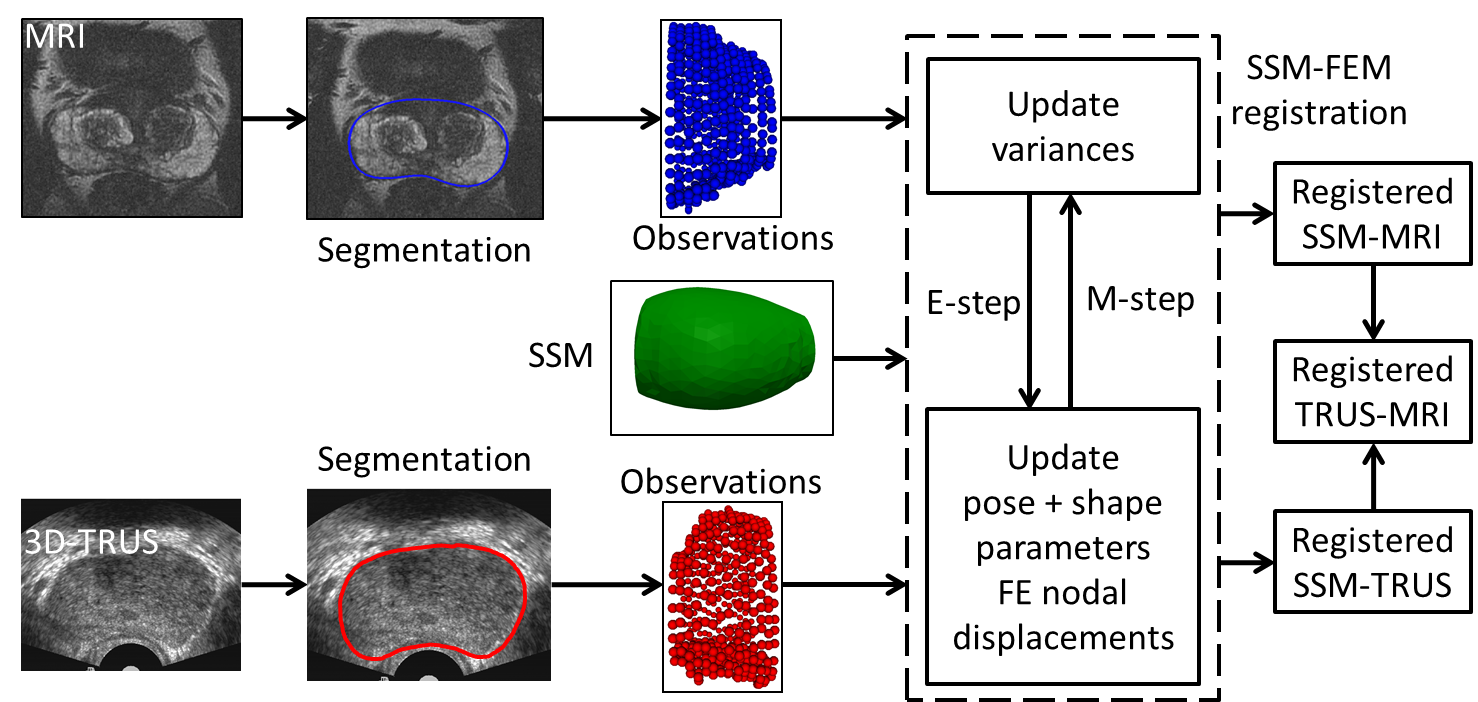
\includegraphics[width = 0.65\textwidth]{images/workflow.png}
\caption{Overview of the registration framework. The pre-operative (MR) image is taken before the procedure and is segmented to create a surface representation of the anatomy, in this case the prostate. At the beginning of the procedure, an intra-operative (3D-TRUS) image is acquired and parts of the anatomy (midgland) are segmented. The SSM-FEM registration maps both surfaces and their interior to the common SSM representation. Subsequently, the MRI is registered to the TRUS space by concatenating MRI-SSM and TRUS-SSM transforms.}
\label{fig:workflow}
\end{figure*}
%%%%%%%%%%%%%%%%%%%%%%%%%%%%%%%%%%%%%%
\section{Method}
%%%%%%%%%%%%%%%%%%%%%%%%%%%%%%%%%%%%%%
An outline of our proposed probabilistic SSM-FEM registration approach is shown in Figure~\ref{fig:workflow}. The partial-surface-to-partial-surface registration is cast as two coupled SSM-to-partial-surface problems, which are solved concurrently using an EM approach. In our formulation, the SSM is used to construct two separate probability density functions (one for each modality) for the boundary of the structure.  These relate the SSM to points on the segmented surface in each modality.  The two segmented surfaces are considered independent sets of observations.  We wish to find:
\begin{enumerate}
	\renewcommand{\theenumi}{\alph{enumi}} % alpha numbering
	\item The single set of SSM modes that best fit \emph{both} partial observations
	\item Two non-rigid transformations (one for each modality) that map the SSM to each observation
\end{enumerate}

To construct the SSM we use a group-wise GMM approach, which has been shown to provide a generally applicable, anatomically specific and compact~\cite{Styner03a} representation of surfaces~\cite{Rasoulian12b}. Details of the training are provided in Section~\ref{sec:ssm}. The result is a linear model, where shapes can be generated from the SSM by adding a linear combination of the modes of variation to the mean shape.  The linear weights, hereafter referred to as \textbf{shape parameters}, along with the modes of variation, define a single \textbf{instance} of the SSM. The parameters that control the rigid transformation of an instance are referred to as \textbf{pose parameters}. During the course of registration, instances of the SSM are used to create a finite element (FE) model of the prostate. This FE model is used to compute internal deformations given a set of boundary conditions. Note that to form an FE model from a surface, we often need to add new nodes interior to the surface. This can be done with most FE-meshing tools, such as TetGen \cite{Si06a}.

Given an SSM, we need to define a probability distribution for the anatomical boundary of interest for each modality.  We use a GMM, which has been widely used to establish soft correspondences~\cite{Myronenko10a,Rasoulian12a,Jian11a}. A GMM is a parametric probability density function represented as a weighted sum of Gaussian densities. Starting from the SSM, we first define a pair of composite transforms that deforms the surface to fit each of the observations.  These are based on a combination of a rigid transform (to account for change in coordinates) and a finite element model which involves some tissue parameters that govern how the prostate is allowed to deform.  The vertices of the deformed SSM are then assumed to be the centroids of Gaussian components, each represented by a mean and a variance. For simplicity, we take the variance to be isotropic in all directions for all components.

The key idea in our registration is that the points on the surface of the prostate in US and MR are deformed observations of a common instance of the SSM. Hence, the solution to the shape parameters depend on both sets of observations. For simplicity, we consider the pose and biomechanical parameters between the SSM and each group of observations to be independent of each other. A full list of notations for the proposed probabilistic SSM-FEM method is presented in Table~\ref{tbl:notation}.
%%%%%%%%%%%%%%%%%%%%%%%%%%%%%%%%%%%%%%
\begin{table}[!bht]
  \centering
  \caption{Mathematical Notations \label{tbl:notation}}
  \begin{tabular}{lp{0.55\columnwidth}}
  \hline
    $\mathrm{md}\in\{\mathrm{US},\mathrm{MR}\}$ & Modality\\
    $D$ & Dimension of the surfaces\\
    $N_\mathrm{md},M,L,J$ & Number of observations in modality, SSM nodes, modes of variation and FEM nodes\\
    $X_\mathrm{md}$ & ${N_\mathrm{md}\times D}$ Observations\\
    $Z_{M\times D}$ & SSM mean\\
    $\Psi_{DM\times L}$ & Modes of variation in rasterized format\\
    $b_{L\times 1}$ & Shape parameters\\
    $R_\mathrm{md},t_\mathrm{md},s_\mathrm{md}$ & $D\times D$ Rotation, $D\times 1$ translation and scale\\
    $Y_{M\times D}$ & An instance of the SSM\\
    $U_\mathrm{md}$ & ${J\times D}$ FEM nodal displacements\\
    $x^\mathrm{md}_n$ & n-th point of observations\\
    $z_m$ & m-th SSM mean node\\
    $y_m$ & m-th instance node\\
    $\vec{v}_{DN \times 1}$ & Rasterized representation of a $V_{N\times D}$ matrix\\
    $\Phi_{M\times J}$ & FEM interpolation matrix\\
    $K$ & Stiffness matrix\\
    $E$ & Young's modulus\\
    $\nu$ & Poisson's ratio\\
    $P_{\mathrm{md}}$ & $M\times N_\mathrm{md}$ GMM posterior probabilities\\ 
    $\sigma_{\mathrm{md}}^2$ & Variance of Gaussian components\\
    $0{\leq}w_{\mathrm{md}}{\leq}1$ & Estimate of outliers/missing data\\
    $\diag{(\vec{v})}$ & Diagonal matrix of a vector $\vec{v}$\\
    $I$ & Identity matrix\\
    $\tilde{P} = \kron{(P,I_{D\times{D}})}$ &Kronecker product of $P$ and $I$\\
    $1$ & Column vector of all ones\\
    \hline\\
  \end{tabular}
\end{table}
%%%%%%%%%%%%%%%%%%%%%%%%%%%%%%%%%%%%%%
\subsection{Probabilistic SSM-FEM}
%%%%%%%%%%%%%%%%%%%%%%%%%%%%%%%%%%%%%%
The probabilistic SSM-FEM registration method, hereafter referred to as SSM-FEM, is based on an EM framework, and is constrained by Tikhonov regularization over shape parameters and the volumetric strain energy of an FE model. The solution is derived by minimizing a single objective functional:
%%%%%%%%%%%%%%%%%%%%%%%%%%%%%%%%%%%%%%
\begin{equation} \label{eq:objTotal1}
\mathcal{E} = \sum_{\mathrm{md}\in\{\mathrm{MR},\mathrm{US}\}}\mathcal{E}_\mathrm{md}(\sigma^2_\mathrm{m},\Theta_\mathrm{md}) + \mathcal{R}_\mathrm{md}(\Theta_\mathrm{md}),
\end{equation}
%%%%%%%%%%%%%%%%%%%%%%%%%%%%%%%%%%%%%%
where $\Theta_\mathrm{md}=(R_\mathrm{md},t_\mathrm{md},s_\mathrm{md},U_\mathrm{md},b)$ is the concatenation of a rigid coordinate transform, nodal displacements, and the single (modality-independent) set of shape parameters. $\mathcal{E}_\mathrm{md}(\cdot)$ is the negative log-likelihood function
%%%%%%%%%%%%%%%%%%%%%%%%%%%%%%%%%%%%%%
\begin{multline} \label{eq:objMod1}
\mathcal{E}_\mathrm{md}(\sigma^2_\mathrm{md},\Theta_\mathrm{md}) = \\ -\sum_{n=1}^{N_\mathrm{md}}\log\sum_{m=1}^MP_\mathrm{md}(z_m)P_\mathrm{md}(x^\mathrm{md}_n|T(z_m,\Theta_\mathrm{md})),
\end{multline}
%%%%%%%%%%%%%%%%%%%%%%%%%%%%%%%%%%%%%%
where $P_\mathrm{md}(\cdot)$ denotes the GMM probability density function~\cite{Myronenko10a} and $T(z_m,\Theta_\mathrm{md})$ represents the transformed location of the $m$-th node in the SSM mean, $z_m$. This transform is defined as:
%%%%%%%%%%%%%%%%%%%%%%%%%%%%%%%%%%%%%%
\begin{equation} \label{eq:concTransform1}
T(z_m,\Theta_\mathrm{md}) = s_\mathrm{md}R_\mathrm{md}(y_m+v^\mathrm{md}_m) + t_\mathrm{md},
\end{equation}
%%%%%%%%%%%%%%%%%%%%%%%%%%%%%%%%%%%%%%
where $y_m=z_m+\Psi_mb$ represents the $m$-th instance node, given shape parameters $b$ and corresponding modes of variation in the columns of $\Psi$. Note that the residual biomechanical deformation between the shape instance and observation, $v^\mathrm{md}_m$, is computed in the SSM space.  This is to reduce rotational artifacts when using a linear material model for the FEM.  Since the SSM is a surface model, we use an interpolation matrix $v^\mathrm{md}_m=\Phi_mU_\mathrm{md}$ to relate surface displacements to nodal displacements. In our implementation, all points on the surface correspond to FE nodes, and internal nodes are appended to the end of the node list. As a result, the interpolation matrix has the form, $\Phi=\begin{bmatrix} I_{M\times M} & 0\\ 0 & 0 \end{bmatrix}$.  In the general case, $\Phi$ would be a sparse matrix which can be computed directly from FE shape functions.  With these substitutions, we can expand Equation~\eqref{eq:concTransform1} as
%%%%%%%%%%%%%%%%%%%%%%%%%%%%%%%%%%%%%%
\begin{equation} \label{eq:concTransform2}
T(z_m,\Theta_\mathrm{md}) = s_\mathrm{md}R_\mathrm{md}(z_m+\Psi_mb+\Phi_mU_\mathrm{md})+t_\mathrm{md}.
\end{equation}
%%%%%%%%%%%%%%%%%%%%%%%%%%%%%%%%%%%%%%
This is the transform used in Equation \eqref{eq:objMod1} that completes the definition of the negative log-likelihood objective functions.  The set of unknowns $\{\sigma^2_\mathrm{md}$, $\Theta_\mathrm{md}\}$ are solved using an EM algorithm. The initial variance is estimated directly from the data as in Myronenko~\textit{et~al.}~\cite{Myronenko10a},
%%%%%%%%%%%%%%%%%%%%%%%%%%%%%%%%%%%%%%
\begin{equation} \label{eq:initVariance}
\sigma^2_\mathrm{md} = \frac{1}{DMN_\mathrm{md}}\sum_{n=1}^{N_\mathrm{md}}\sum_{m=1}^{M}\left\|x^{\mathrm{md}}_n-z_m\right\|^2.
\end{equation}
%%%%%%%%%%%%%%%%%%%%%%%%%%%%%%%%%%%%%%
In the expectation step, we compute how likely an observation corresponds to a GMM centroid by calculating the posterior probability
%%%%%%%%%%%%%%%%%%%%%%%%%%%%%%%%%
\begin{align} \label{eq:prob}
P_\mathrm{md}(z_m|x^\mathrm{md}_n) = & \frac{\exp{\left(-\frac{1}{2}\frac{\left\|x^\mathrm{md}_n -T(z_m,\Theta_\mathrm{md})\right\|^2}{\sigma^2_\mathrm{md}}\right)}}{\sum_{j=1}^M\exp{\left(-\frac{1}{2}\frac{\left\|x_n -T(z_j,\Theta_\mathrm{md})\right\|^2}{\sigma^2_\mathrm{md}}\right)} + c},
\end{align}
where 
\begin{align}
c = & \left(2\pi\sigma^2_\mathrm{md}\right)^{D/2}\frac{w_\mathrm{md}}{1-w_\mathrm{md}}\frac{M}{N_\mathrm{md}}
\end{align}
%%%%%%%%%%%%%%%%%%%%%%%%%%%%%%%%%
%where $c=(2\pi\sigma^2_\mathrm{md})^{D/2}\frac{w_\mathrm{md}}{1-w_\mathrm{md}}\frac{M}{N_\mathrm{md}}$ 
is the contribution of an additional uniform distribution to account for noise, outliers and missing data. The scalar weight $0{\leq}w_\mathrm{md}{\leq}1$ controls equal membership probabilities, set to zero if observations do not exhibit any noise, outliers or missing data. A value of one denotes that no correspondence between observations and GMM centroids can be made. Ignoring terms independent of $\sigma^2_\mathrm{md}$ and $\Theta_\mathrm{md}$, we can rewrite the negative log-likihood function of Equation~\eqref{eq:objMod1} as
%%%%%%%%%%%%%%%%%%%%%%%%%%%%%%%%%
\begin{multline} 
\hat{\mathcal{E}}_\mathrm{md}(\sigma^2_\mathrm{md},\Theta_\mathrm{md}) = \frac{N^\mathrm{md}_PD}{2}\log(\sigma^2_\mathrm{md})\\
\quad\quad + \frac{1}{2\sigma^2_\mathrm{md}}\sum_{m,n=1}^{M,N_\mathrm{md}}P_\mathrm{md}(z_m|x^\mathrm{md}_n)\left\|x^\mathrm{md}_n- T(z_m,\Theta_\mathrm{md})\right\|^2, \label{eq:Emd}
\end{multline}
where $N^\mathrm{md}_P=\sum_{m,n=1}^{M,N_\mathrm{md}}P_\mathrm{md}(z_m|x^\mathrm{md}_n)$.  To contrain the SSM shape parameters and the FE nodal displacements, we add the Tikhonov regularizers:
\begin{align} \label{eq:Rmd}
\mathcal{R}_\mathrm{md}(\Theta_\mathrm{md}) = \frac{\mu}{4}\trans{b}\Lambda{b} + \frac{\beta}{2}\trans{\vec{u}_\mathrm{md}}K\vec{u}_\mathrm{md}. 
\end{align}
%%%%%%%%%%%%%%%%%%%%%%%%%%%%%%%%%
The $\mu$ parameter controls the regularization of shape parameters, with $\Lambda$ the diagonal matrix of inverted SSM eigenvalues. This term is scaled by $1/4$ since it is split equally between the two observations.  If we were registering $n$ observations, the fraction would be $1/2n$. The $\beta$ parameter controls the trade-off between tightness of the fit and biomechanical regularization. This term represents the total linearized strain energy of the FE model \cite{Bonet00a}.  It involves the \emph{stiffness matrix}, $K$, and a rasterized vector of nodal displacements, $\vec{u}$.  The stiffness matrix is a large sparse matrix that can be systematically constructed based on the FE mesh and the material parameters.  For simplicity, we assume a linear stress-strain relationship.  More complex material models can be applied, but the linearized strain-energy will then include an additional forcing term dependent on the current deformation state.  In the current implementation, whenever the SSM is updated, we remesh the FE model to ensure a high mesh quality.  Substituting Equations~\eqref{eq:Emd} and \eqref{eq:Rmd} into Equation~\eqref{eq:objTotal1} yields the total objective function to be minimized:
%%%%%%%%%%%%%%%%%%%%%%%%%%%%%%%%%
\begin{equation} \label{eq:objTotal2}
\mathcal{E} = \sum_{\mathrm{md}\in\{\mathrm{MR},\mathrm{US}\}}\hat{\mathcal{E}}_{\mathrm{md}}(\sigma^2_\mathrm{md},\Theta_\mathrm{md}) + \mathcal{R}_\mathrm{md}(\Theta_\mathrm{md}).
\end{equation}
%%%%%%%%%%%%%%%%%%%%%%%%%%%%%%%%%

To perform the registration, we need to minimize the total objective function in Equation \eqref{eq:objTotal2}.  Unfortunately, due to the coupling between the rigid transforms, FEM deformation, and shape parameters, finding the optimal solution to this objective function directly is non-trivial.  Instead, we propose a simple alternating minimization strategy.  First, we assume that the FEM deformation and SSM shape parameters are fixed, and solve for the pose parameters of each observation: $\{R_\mathrm{md},t_\mathrm{md}, s_\mathrm{md}\}$.  Since each observation is assumed independent, this results in a pair of rigid registration problems between pairs of surfaces.  The formulation is precisely the ``rigid'' coherent point drift problem detailed by and solved in Myronenko~\textit{et~al.}~\cite{Myronenko10a}.  After this step, the current estimate of each deformed model is best aligned to the observations.

The next step of the minimization is to update the estimated intermediate shape from the SSM.  This requires finding the solution to the optimum shape parameters, $b$, which is dependent on \textit{all} observations.  The solution given one observation is outlined in~\cite{Rasoulian12b}. By extension, (see Appendix~\ref{sec:app:ssm}) the optimum shape parameters provided two sets of observations is the solution to the following set of linear equations:
%%%%%%%%%%%%%%%%%%%%%%%%%%%%%%%%%%%%%%
\begin{equation} \label{eq:SSM1}
\Gamma_{\mathrm{SSM}}b = \Upsilon_\mathrm{SSM},
\end{equation}
%%%%%%%%%%%%%%%%%%%%%%%%%%%%%%%%%%%%%%
with
%%%%%%%%%%%%%%%%%%%%%%%%%%%%%%%%%%%%%%
\begin{align} \label{eq:SSM2}
\Gamma_{\mathrm{SSM}} = & \mu\Lambda + \sum_\mathrm{md}\frac{s^2_\mathrm{md}}{\sigma^2_\mathrm{md}}\trans{\Psi}\diag(\tilde{P}_\mathrm{md}1)\Psi,\\
 \Upsilon_{\mathrm{SSM}} = & \sum_{\mathrm{md}}\frac{s_\mathrm{md}}{\sigma^2_\mathrm{md}}\left(\trans{\Psi}\trans{\tilde{R}}_\mathrm{md}\tilde{P}_\mathrm{md}\vec{x}_\mathrm{md}\right.\nonumber\\
 & \;\; \left.-\trans{\Psi}\diag(\tilde{P}_\mathrm{md}1)\!\left(s_\mathrm{md}(\vec{z}+\vec{v}_\mathrm{md})+\tilde{I}\trans{R}_\mathrm{md}t_\mathrm{md}\right)\right)\nonumber.
\end{align}
%%%%%%%%%%%%%%%%%%%%%%%%%%%%%%%%%%%%%%
The resulting shape instance can be thought of as a common ``starting shape'', from which we will determine further biomechanical deformation for each of the observations.

Finally, we compute FE nodal displacements, keeping the pose and shape parameters fixed.  A single finite element model is automatically generated from the SSM shape instance.  For this, we generate a volumetric tetrahedral mesh using TetGen \cite{Si06a}, and assume a linear material model.  Since the observations are considered independent, displacements can be solved independently for each input modality. Minimizing Equation~\eqref{eq:objTotal2} with respect to the rasterized vector $\vec{u}_\mathrm{md}$ yields the following sparse set of linear equations:
%%%%%%%%%%%%%%%%%%%%%%%%%%%%%%%%%%%%%%
\begin{equation} \label{eq:FEM1}
\Gamma_{\mathrm{FEM}}\vec{u}_\mathrm{md} = \Upsilon_\mathrm{FEM},
\end{equation}
%%%%%%%%%%%%%%%%%%%%%%%%%%%%%%%%%%%%%%
where 
%%%%%%%%%%%%%%%%%%%%%%%%%%%%%%%%%%%%%%
\begin{eqnarray} \label{eq:FEM2}
 \Gamma_{\mathrm{FEM}} &=& \beta \sigma_\mathrm{md}^2K + s^2_\mathrm{md}\trans{\tilde{\Phi}}\diag(\tilde{P}_\mathrm{md}1)\tilde{\Phi}\\
 \Upsilon_{\mathrm{FEM}} &=& s_\mathrm{md}\trans{\tilde{\Phi}}\trans{\tilde{R}}_\mathrm{md}\tilde{P}_\mathrm{md}\vec{x}_\mathrm{md}\nonumber\\
 && -\trans{\tilde{\Phi}}\diag(\tilde{P}_\mathrm{md}1)\left(s_\mathrm{md}^2\vec{y}+s_\mathrm{md}\tilde{I}\trans{R_\mathrm{md}}t_\mathrm{md}\right)\nonumber.
\end{eqnarray}
%%%%%%%%%%%%%%%%%%%%%%%%%%%%%%%%%%%%%%
Full details of the derivation are provided in Appendix~\ref{sec:app:fem}.  The nodal displacements, $\vec{u}_\mathrm{md}$, can be easily determined using any sparse linear solver.  At the end of this step, we have now updated all unknown parameters required by the transformation function \eqref{eq:concTransform2}. 

With the transformation from the SSM to each set of observations known, we can recalculate the estimated variances, $\sigma^2_\mathrm{md}$. This step is exactly as Myronenko~\textit{et~al.}~\cite{Myronenko10a} and is presented here for completeness:
%%%%%%%%%%%%%%%%%%%%%%%%%%%%%%%%%%%%%%
\begin{equation} \label{eq:max1}
\sigma^2_\mathrm{md} = \frac{1}{N^\mathrm{md}_p}\sum^{M,N_\mathrm{md}}_{m,n=1}\left\|x^{\mathrm{md}}_n-T(z_m,\Theta_\mathrm{md})\right\|^2.
\end{equation}
%%%%%%%%%%%%%%%%%%%%%%%%%%%%%%%%%%%%%%
With this new variance estimate, we can update the GMM probability distributions (Equation \eqref{eq:prob}).

The registration algorithm iterates between the expectation step (updating GMM distributions) and maximization step (updating the transform parameters) until the variances drop below a certain threshold. The complete algorithm for the proposed SSM-FEM registration is summarized in Algorithm~\ref{alg:SSMFEM1}.
%%%%%%%%%%%%%%%%%%%%%%%%%%%%%%%%%%%%%%
\begin{algorithm}[t]\label{alg:SSMFEM1}
 \SetAlgoLined
 Require: $E$, $\nu$, $\mu$, $\beta$, $Z$, $\Psi$, $X_\mathrm{md}$ and $w_\mathrm{md}$\;
 Initialize: $b$, $s_\mathrm{md}$, $R_\mathrm{md}$, $t_\mathrm{md}$, $\vec{u}_\mathrm{md}$ and $\sigma^2_\mathrm{md}$\;
 where $\mathrm{md}\in\{\mathrm{MR},\mathrm{US}\}$\;
 \While{not converged}{
  E-Step:\newline
  {
     \For{$\mathrm{md}\in\{\mathrm{MR},\mathrm{US}\}$}{
     Update $P_\mathrm{md}$ using Equation~\eqref{eq:prob};
     }
  }
  % \phantom{\ }
  M-Step:\newline
  {
     \For{$\mathrm{md}\in\{\mathrm{MR},\mathrm{US}\}$}{
     Rigid registration between $X_\mathrm{md}$ and $Y+{\Phi}U_\mathrm{md}$\;
     Update pose: $s_\mathrm{md}$, $R_\mathrm{md}$ and $t_\mathrm{md}$\;
     }

     Shape registration using Equation~\eqref{eq:SSM1}\;
     Update $b$ which updates $Y$\;
     \For{$\mathrm{md}\in\{\mathrm{MR},\mathrm{US}\}$}{
     Biomechanical registration using Equation~\eqref{eq:FEM1}\;
     Update $U_\mathrm{md}$\;
     }
     \For{$\mathrm{md}\in\{\mathrm{MR},\mathrm{US}\}$}{
     Update $\sigma^2_\mathrm{md}$ using Equation~\eqref{eq:max1};
     }
    }
 }
 \caption{SSM-FEM registration \label{alg:registration}}
\end{algorithm}
%%%%%%%%%%%%%%%%%%%%%%%%%%%%%%%%%%%%%%

Once the SSM-FEM registration has converged, we can propagate the FEM using $\Theta_\mathrm{md}$ into the space of the TRUS and MR images. This enables us to express voxels in either modality using the natural coordinates of the FEM. Thus, for voxels inside the prostate in one modality, it is possible to find its corresponding voxel in the other modality.

For biomechanical material properties, we apply a homogeneous elastic material with a constant Young's modulus to all elements.  The models used in this study are composed of $\approx7500$ elements. Throughout our experiments, we used a stopping condition of $\sigma^2\leq1e^{-4}~\mathrm{mm}^2$, Young's modulus of $E=5$~kPa, which is in the range of values reported in~\cite{Kemper04a} for the prostate, and a Poisson's ratio of $\nu=0.49$.
%%%%%%%%%%%%%%%%%%%%%%%%%%%%%%%%%%%%%%
\subsection{Registration Methods Used for Comparison}
%%%%%%%%%%%%%%%%%%%%%%%%%%%%%%%%%%%%%%
The proposed SSM-FEM registration method consists of two priors: 1) Geometrical (SSM); and 2) Biomechanical (FEM). In order to highlight the importance of each component, we compare the proposed method by removing each \textit{a priori} piece of information. By keeping only the geometrical prior, we are implicitly assuming that the SSM, TRUS and MR surfaces are in the same biomechanical state. The concurrent registration of a SSM to TRUS and MR surfaces without the biomechanical component is equivalent to a rigid registration of MR and TRUS surfaces. Henceforth, we refer to this approach as SSM registration.

%%%%%%%%%%%%%%%%%%%%%%%%%%%%%%%%%
\begin{figure}[t]
	\centering
	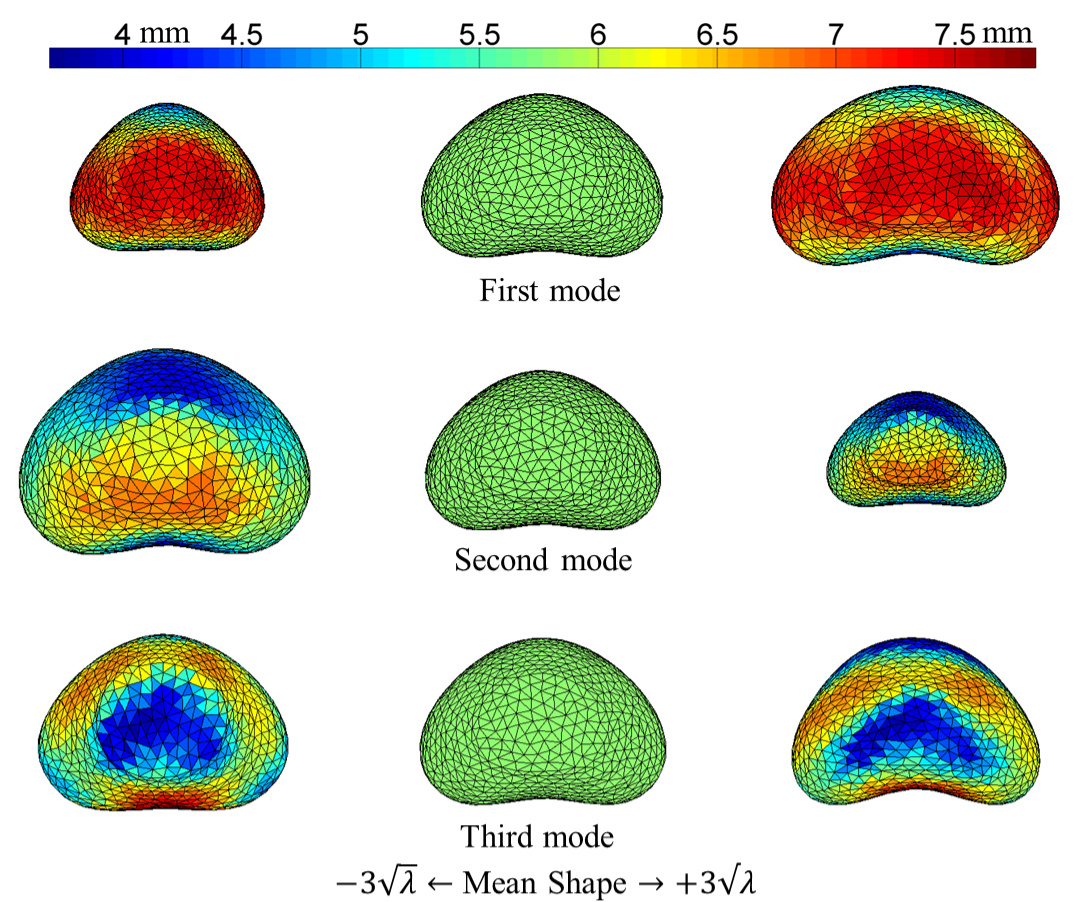
\includegraphics[width=\columnwidth]{images/SSM_modes_inferior}
	\caption{Graphical representation of the prostate shapes described by the SSM after varying weights corresponding to the first three principal modes of variation by three standard deviations ($3\sqrt{\lambda})$. The mean shape is shown with a green model in the middle column. The amount of variation in the left and right column is color coded for each mode.}\label{fig:SSM_modes}
\end{figure}
%%%%%%%%%%%%%%%%%%%%%%%%%%%%%%%%%

If a full surface of the prostate is available, e.g.~through a full segmentation of the MRI, then the need for the geometrical prior is removed. In this case, we can treat the full surface as the source shape instance, and solve only for the coordinate transform and biomechanical deformations between source and target surfaces using Equation~\eqref{eq:FEM1}. We refer to this approach as GMM-FEM registration.  The displacements in this case can be determined by solving the linear system
%%%%%%%%%%%%%%%%%%%%%%%%%%%%%%%%%%%%%%
\begin{equation} \label{eq:GMMFEM1}
\Gamma\vec{u} = \Upsilon,
\end{equation}
%%%%%%%%%%%%%%%%%%%%%%%%%%%%%%%%%%%%%%
where $P,\sigma^2$ describes a GMM that corresponds to the fully segmented source surface and
%%%%%%%%%%%%%%%%%%%%%%%%%%%%%%%%%%%%%%
\begin{eqnarray} \label{eq:GMMFEM2}
 \Gamma &=& \beta \sigma^2K + s^2\trans{\tilde{\Phi}}\diag(\tilde{P}1)\tilde{\Phi}\\
 \Upsilon &=& s\trans{\tilde{\Phi}}\trans{\tilde{R}}\tilde{P}\vec{x}_\mathrm{target}\nonumber\\
 && -\trans{\tilde{\Phi}}\diag(\tilde{P}1)\left(s^2\vec{y}_\mathrm{source}+s\tilde{I}\trans{R}t\right)\nonumber.
\end{eqnarray}
The rest of the algorithm proceeds as usual.

%%%%%%%%%%%%%%%%%%%%%%%%%%%%%%%%%%%%%%
\section{Experiments and Results}
%%%%%%%%%%%%%%%%%%%%%%%%%%%%%%%%%
We evaluate the proposed registration method in a series of experiments with MR-TRUS image pairs acquired from patients who underwent a prostate intervention. The data acquisition protocol was approved by our institutional ethics boards, and all patients provided written consent to be included in the study. The rest of this section is divided into four subsections. In Section~\ref{sec:ssm}, we discuss the training population used for SSM construction. In Section~\ref{sec:biopsy}, we discuss the biopsy data acquisition, segmentation protocol, and the initialization of the registration. Finally, in Section~\ref{sec:exp1}, we validate the accuracy of our registration method by measuring the TRE between pairs of intrinsic fiducials found in the interior of the prostate. To highlight the importance of the SSM, we compare the outcome of the combined SSM-FEM registration with the similar registration that excludes either the SSM or FEM components. In Section~\ref{sec:exp2}, we investigate the sensitivity of our approach to missing observations. Finally, in Section~\ref{sec:exp3}, we investigate sensitivity to free parameters that control the regularization terms in the registration.
%%%%%%%%%%%%%%%%%%%%%%%%%%%%%%%%%

\subsection{Data}
%%%%%%%%%%%%%%%%%%%%%%%%%%%%%%%%%
\subsubsection{SSM Construction}\label{sec:ssm}
%%%%%%%%%%%%%%%%%%%%%%%%%%%%%%%%%
One of the underlying assumptions of our procedure is that we have an SSM that represents the inter-subject variation of prostate shapes.  To construct such a statistical model, a suitable choice for training data is a large population of prostate images that are acquired using the same modality. The choice of the imaging modality is important, since biomechanical forces (e.g.~from end-firing probes and endorectal coils) affect the shape of the prostate in TRUS and MRI, respectively. Ideally, the prostates should be in the same biomechanical deformation state, so that differences in appearance are mostly due to inter-subject variations. Finally, for surface-based SSMs, the prostate needs to be accurately and reliably segmented.

Brachytherapy volumes are routinely acquired and segmented in large clinics and interventional centers. We used a dataset of images aquired from 290 brachytherapy patients in the construction of our SSM. Each TRUS volume consists of 7 to 14 parallel equally spaced ($5$~mm apart) axial B-mode images of the prostate which are captured using a side-firing transrectal probe. For each B-mode image, the prostate gland is delineated using Variseed (Varian Medical Systems, Palo~Alto, CA, USA) and a contouring plug-in. This plug-in is based on the semi-automatic prostate segmentation method presented by Mahdavi~\textit{et al.}~\cite{Mahdavi11a}. These contours are manually corrected by an expert clinician, and subsequently used as the training population in our SSM construction.

As mentioned previously, we used the group-wise GMM method~\cite{Rasoulian12b} for the construction of the SSM. This resulted in a SSM with a mean shape consisting of 1000 nodes and 1996 faces. The mean and primary modes of variation are depicted in Figure~\ref{fig:SSM_modes}. As seen in the figure, the first two modes control the scale, whereas the third mode controls the curvature of the prostate.

%%%%%%%%%%%%%%%%%%%%%%%%%%%%%%%%%
\begin{figure}[t]
	\centering
	\subfloat[][Base\label{fig:MRData1}]{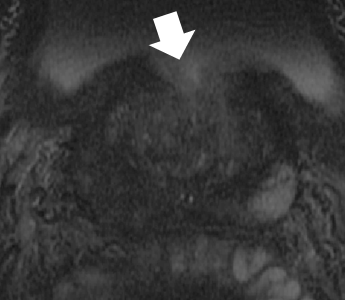
\includegraphics[width=0.33\columnwidth,height=1.2in]{images/MRData1}} \hfill
	\subfloat[][Mid-gland\label{fig:MRData2}]{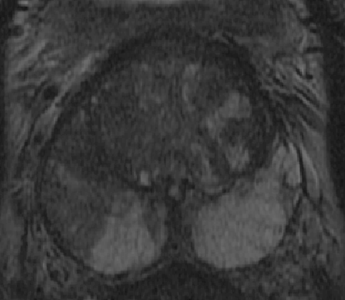
\includegraphics[width=0.33\columnwidth,height=1.2in]{images/MRData2}} \hfill
	\subfloat[][Apex\label{fig:MRData3}]{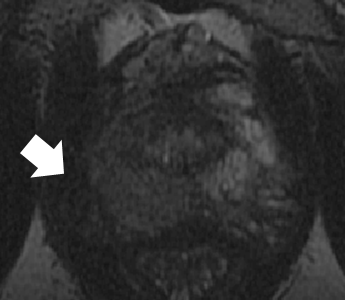
\includegraphics[width=0.33\columnwidth,height=1.2in]{images/MRData3}}\\
	\subfloat[][Base\label{fig:TRUSData1}]{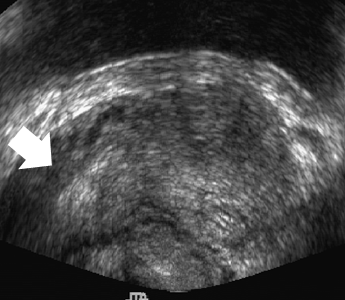
\includegraphics[width=0.33\columnwidth,height=1.2in]{images/USData1}} \hfill
	\subfloat[][Mid-gland\label{fig:TRUSData2}]{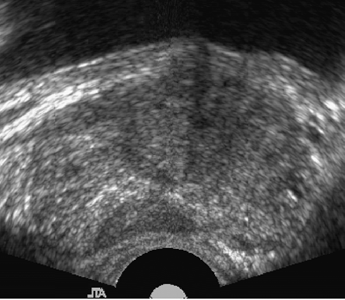
\includegraphics[width=0.33\columnwidth,height=1.2in]{images/USData2}} \hfill
	\subfloat[][Apex\label{fig:TRUSData3}]{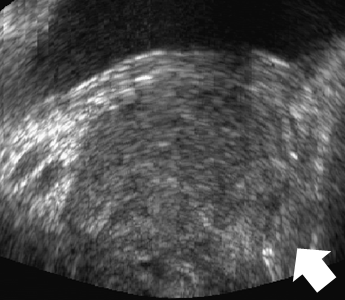
\includegraphics[width=0.33\columnwidth,height=1.2in]{images/USData3}}\\
	\hspace*{0.75cm}
	\subfloat[][MR Segmentation\label{fig:MRSeg}]{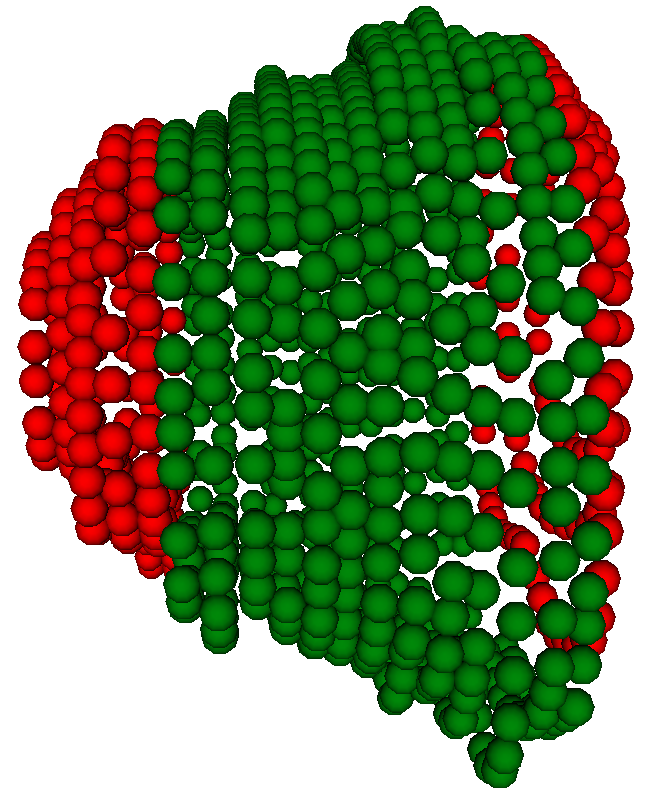
\includegraphics[width=0.33\columnwidth]{images/MR_Segmentation}}\hfill
	\subfloat[][TRUS Segmentation\label{fig:TRUSSeg}]{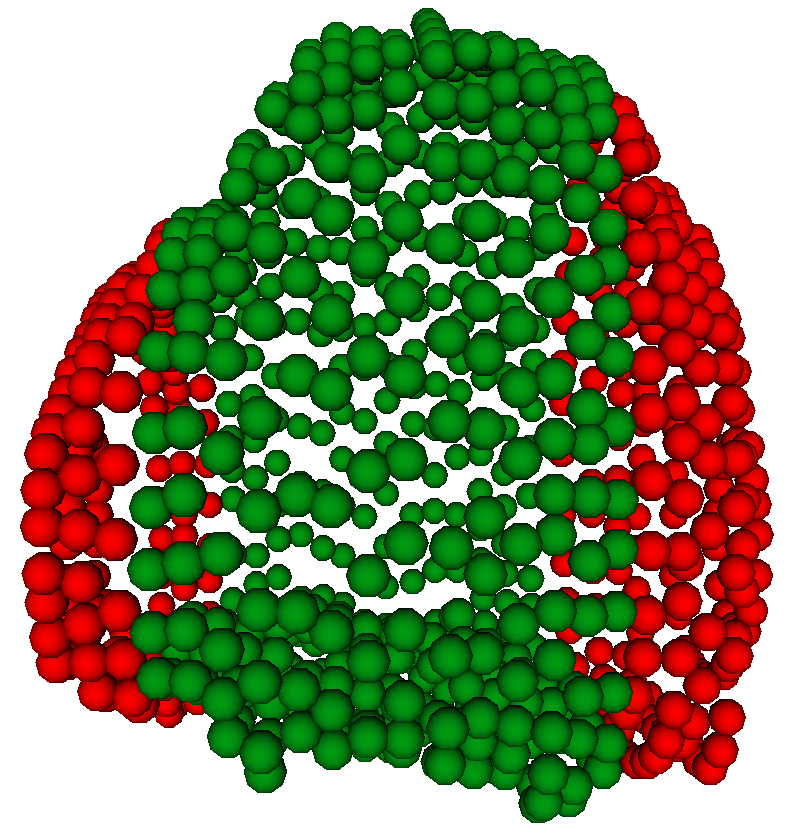
\includegraphics[width=0.33\columnwidth]{images/TRUS_Segmentation}}
	\hspace*{0.75cm}
  \caption{Axial slices from MR (top-row) and TRUS (middle-row) volumes. Typically, the prostate boundary can be accurately and reliably segmented in the mid-gland, i.e. (b) and (e). White arrows highlight regions where the true prostate boundary is ambiguous. (g) and (h) depict the resulting segmentation of MR and TRUS, respectively. Partial segmentations are color coded in green, uncertain contours are in red.}\label{fig:biopsy1}
\end{figure}
%%%%%%%%%%%%%%%%%%%%%%%%%%%%%%%%%

The choice of the number of modes is governed by the compactness of the SSM. Compactness simply measures the cumulative variance of the model as modes are added in order of descending eigenvalues~\cite{Heimann09a}. A popular general rule is to keep the first $L$ modes that span 95\% of the total variation. For our SSM, this results in a model with 50 principal modes.
%%%%%%%%%%%%%%%%%%%%%%%%%%%%%%%%%
\subsubsection{Prostate Biopsy}\label{sec:biopsy}
%%%%%%%%%%%%%%%%%%%%%%%%%%%%%%%%%
The validation data was acquired from ten patients scheduled for a prostate biopsy. In Figure~\ref{fig:biopsy1}, a typical example MR and TRUS images is shown. The T2-weighted MR images were acquired using a 3 Tesla GE Excite HD MRI system (Milwaukee, WI, USA) with a spacing of $0.27~\times~0.27~\times~2.2$ mm. Typical slices from base, mid-gland and apex are shown in Figures~\ref{fig:MRData1},\ref{fig:MRData2} and \ref{fig:MRData3}, respectively. The TRUS images were acquired using a 3D-TRUS mechanical biopsy system~\cite{Bax08a} with a Philips HDI-5000 US machine and a C9-5 transducer using an axial rotation of the biopsy probe. The TRUS images were reconstructed into a 3D-volume with a spacing of $0.19~\times~0.19~\times~0.19$ mm. Figures~\ref{fig:TRUSData1},\ref{fig:TRUSData2} and \ref{fig:TRUSData3} show typical slices from base, mid-gland and apex, respectively. In each modality, areas around the mid-gland (e.g. Figures~\ref{fig:MRData2} and \ref{fig:TRUSData2}) were segmented where the prostate boundary could be reliably and accurately traced. We refer to these contours as a \textbf{partial} segmentation. Additionally, we segmented regions of the prostate where the prostate boundary was not easily visible, i.e. base and apex, using symmetry and prior knowledge of the general ellipsoid-like shape of the prostate. The white arrows in Figure~\ref{fig:biopsy1} indicate examples of these uncertain regions. The prostate contours extracted from these uncertain regions are referred to as \textbf{uncertain} data. The combination of both uncertain and partial data is referred to as the \textbf{full} data. Example segmentations of MR and TRUS volumes are shown in Figures~\ref{fig:MRSeg} and \ref{fig:TRUSSeg}, respectively. To initialize the registration, the full prostate surfaces from the MRI and TRUS are brought to an initial position with respect to the mean SSM shape using right-anterior-superior (RAS) coordinates and center of mass alignment.
%%%%%%%%%%%%%%%%%%%%%%%%%%%%%%%%%
\subsection{Registration of Full and Partial Surfaces}\label{sec:exp1}
%%%%%%%%%%%%%%%%%%%%%%%%%%%%%%%%%
\begin{figure}[t]
	\centering
	\subfloat[][Initial\label{fig:InitFull}]{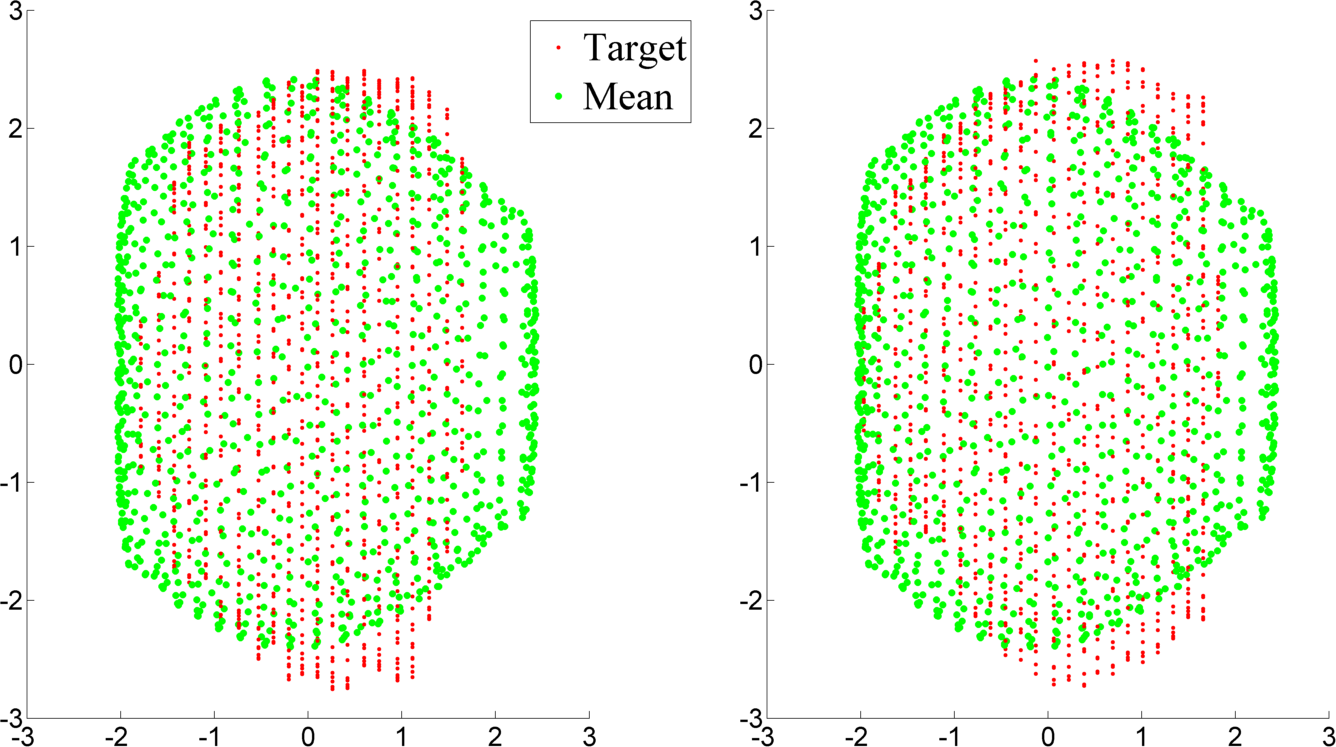
\includegraphics[width=0.95\columnwidth]{images/SSM_FEM_Full_Initial}}\\
	\subfloat[][Registered\label{fig:Resultfull}]{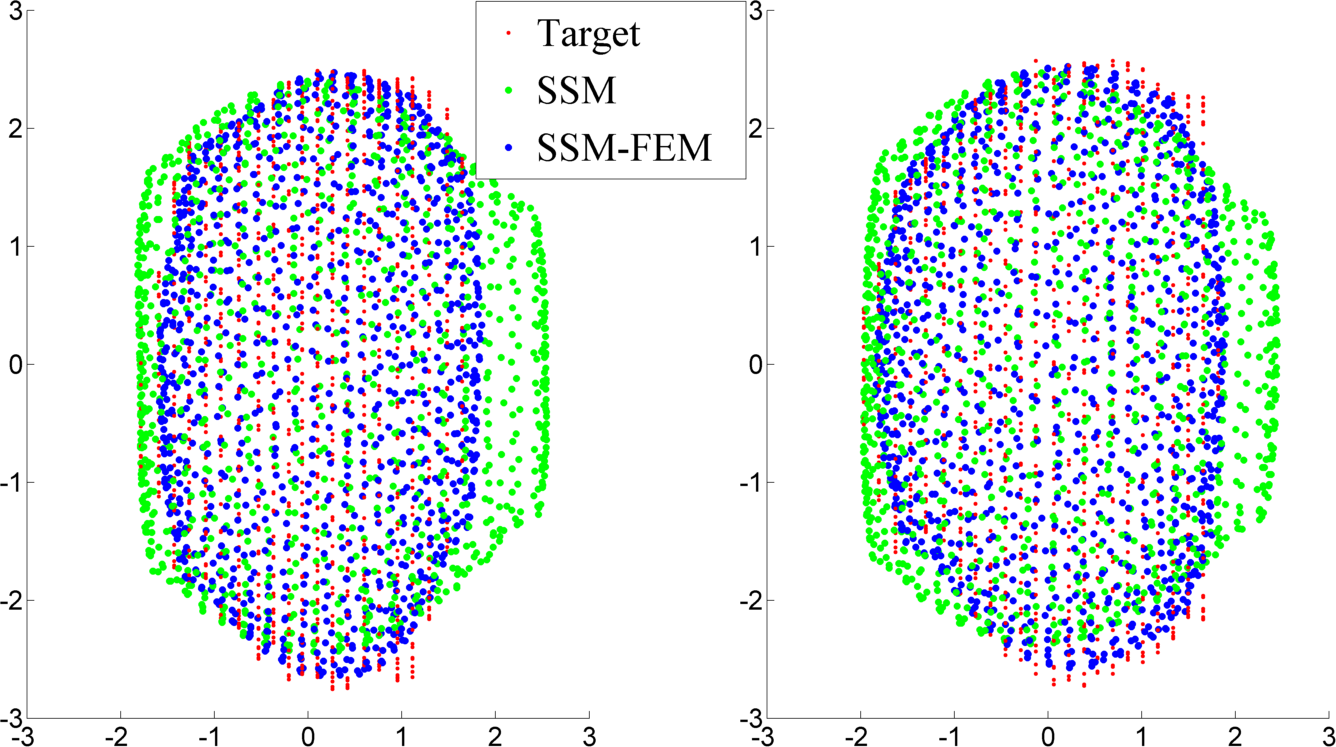
\includegraphics[width=0.95\columnwidth]{images/SSM_FEM_Full_Registered}}
	\caption{An example of SSM-FEM registration with $w=0.0$, $\mu=400$, $\beta=10.0$, $E=5.0$~kPa and $\nu=0.49$ to full data (TRUS on the left, MR on the right).  Following center of mass initialization (a), the SSM mean is evolved to target surfaces (b). The target surfaces are shown in red, the current SSM instance is shown in green, and the result of SSM-FEM registration is shown in blue.}\label{fig:RegFull}
\end{figure}
%%%%%%%%%%%%%%%%%%%%%%%%%%%%%%%%%
As a first set of experiments, we used the biopsy data described in Section~\ref{sec:biopsy} to validate our registration pipeline using both the pair of full surfaces, and the pair of partial surfaces. Following center of mass initialization between the SSM-mean and target surfaces, as seen in Figure~\ref{fig:InitFull}, we apply the SSM-FEM algorithm until registration converges.  A typical result to using full MR-TRUS surfaces is shown in Figure~\ref{fig:Resultfull}. The Tikhonov regularization weights were tuned such that the best visual surface overlap was achieved. This resulted in a choice of $\mu=400$ and $\beta=10$. Since full surfaces do not have any missing points, we set the estimate of missing data, $w_\mathrm{md}$, to zero throughout this experiment. To maintain a fair comparison, we used the same parameters for SSM and for GMM-FEM registration methods as well.

%%%%%%%%%%%%%%%%%%%%%%%%%%%%%%%%%
\begin{figure}[t]
	\centering
	\subfloat[][Initial\label{fig:InitPartial}]{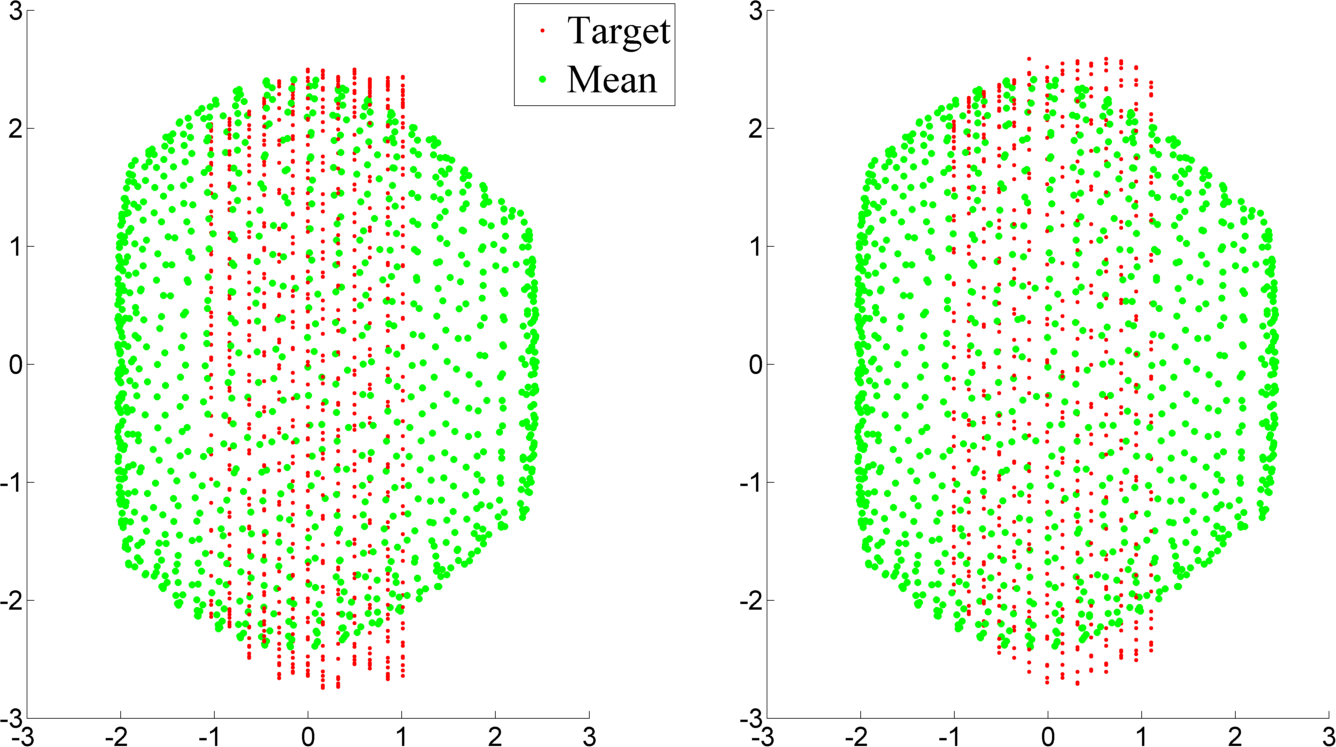
\includegraphics[width=0.95\columnwidth]{images/SSM_FEM_Partial_Initial}}\\
	\subfloat[][Registered\label{fig:ResultPartial}]{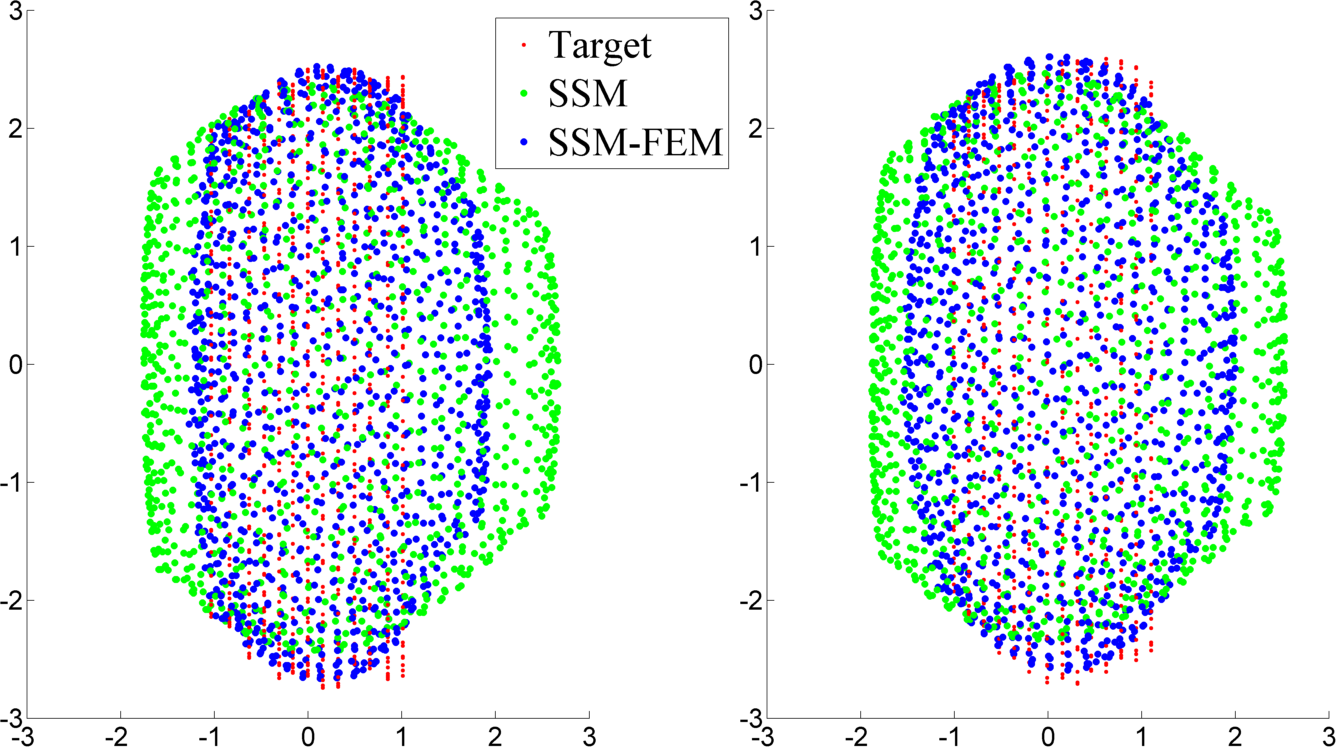
\includegraphics[width=0.95\columnwidth]{images/SSM_FEM_Partial_Registered}}
	\caption{An example of SSM-FEM registration with $w=0.2$, $\mu=400$, $\beta=10.0$, $E=5.0$~kPa and $\nu=0.49$ to partial data (TRUS on the left, MR on the right). Following center of mass initialization (a), the SSM mean is evolved to target surfaces (b). The target surfaces are shown in red, the current SSM instance is shown in green, and the result of SSM-FEM registration is shown in blue.}\label{fig:RegPartial}
\end{figure}
%%%%%%%%%%%%%%%%%%%%%%%%%%%%%%%%%
The same experiment was applied using the partial MR and TRUS surfaces.  A typical SSM-FEM registration result for a partial MR-TRUS surface pair is shown in Figure~\ref{fig:RegPartial}. We used the same Tikhonov regularization weights as for the full data. However, since partial surfaces exhibit missing points, we set the estimate of missing data $w_\mathrm{md}=0.2$. To maintain a fair comparison, the same parameters were used for SSM and GMM-FEM registration methods.
%%%%%%%%%%%%%%%%%%%%%%%%%%%%%%%%%
\subsubsection{Quantitative Validation}
%%%%%%%%%%%%%%%%%%%%%%%%%%%%%%%%%
\begin{figure}[t]
	\centering
	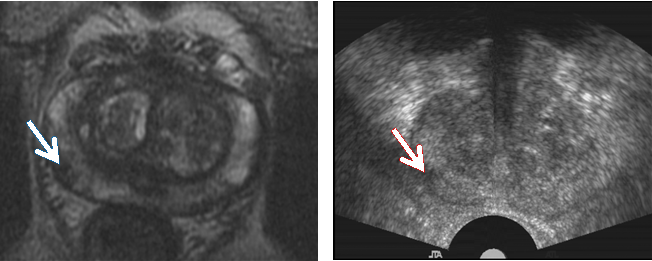
\includegraphics[width=\columnwidth]{images/FiducialPair}
	\caption{Examples of fiducial pairs in MR (left) and TRUS (right) images.}\label{fig:Fiducial}
\end{figure}
%%%%%%%%%%%%%%%%%%%%%%%%%%%%%%%%%
Our registration algorithm was implemented in MATLAB\textregistered\ (MathWorks, MA), and converges within $\approx30$~seconds on a $3.4$~GHz Intel Core i7 CPU with $8.00$~GB of RAM. In order to quantify the registration results, we asked an expert radiologist to select five intrinsic fiducials per patient consisting of cysts and benign prostatic hyperplasia (BPH). Figure~\ref{fig:Fiducial} shows an example of corresponding fiducial pairs in MR and TRUS. The $L_2$ distance between these fiducial pairs was used to quantify the TRE.

%%%%%%%%%%%%%%%%%%%%%%%%%%%%%%%%%
\begin{table}[t]
\begin{center}
\caption{TRE (mm) for center of mass alignment (initial), SSM, GMM-FEM and SSM-FEM registration. The $p$-values reflect Wilcoxon signed-rank tests between initial and subsequent registration.}
\centering
\begin{tabular}{c| c| c| c| c}
	\hline
	& \multicolumn{2}{c|}{TRE} & \multicolumn{2}{c}{$p$-value}\\
	\cline{2-3}  \cline{4-5}
	Method & Full & Partial & Full & Partial \\
	\hline
	Initial & $4.51 \pm 1.21$ & $4.73 \pm 1.31$ & NA & NA \\
	\hline
	SSM & $3.72 \pm 1.17$ & $4.09 \pm 1.63$ & $\eng{1}{-2}$ & $0.33$ \\
	\hline
	GMM-FEM & $2.63 \pm 1.05$ & $5.05 \pm 1.56$ & $\eng{1}{-3}$ & $0.27$ \\
	\hline
	SSM-FEM & $2.56 \pm 0.93$ & $2.95 \pm 0.55$ & $\eng{1}{-4}$ & $\eng{1}{-4}$ \\
   \hline
\end{tabular}
\label{tab:TRE}
\end{center}
\end{table}

%%%%%%%%%%%%%%%%%%%%%%%%%%%%%%%%%
\begin{table}[t]
\begin{center}
\caption{Wilcoxon signed-rank tests between the SSM-FEM registration and methods used for comparison.}
\centering
\begin{tabular}{c| c| c}
	\hline
	& \multicolumn{2}{c}{$p$-value}\\
	\cline{2-3}
	Test & Full & Partial\\
	\hline
	SSM & $\eng{1}{-6}$ & $\eng{1}{-5}$ \\
	\hline
	GMM-FEM & 0.45 & $\eng{1}{-4}$ \\
   \hline
\end{tabular}
\label{tab:stat1}
\end{center}
\end{table}
%%%%%%%%%%%%%%%%%%%%%%%%%%%%%%%%%
\begin{table}[t]
\begin{center}
\caption{Wilcoxon signed-rank tests between full and partial segmentations for each registration method.}
\centering
\begin{tabular}{c| c}
	\hline
	Test & $p$-value\\
	\hline
	SSM & 0.25\\
	\hline
	GMM-FEM & $\eng{1}{-3}$\\
	\hline
	SSM-FEM & 0.33\\
   \hline
\end{tabular}
\label{tab:stat2}
\end{center}
\end{table}

%%%%%%%%%%%%%%%%%%%%%%%%%%%%%%%%%

The mean and standard deviation of the TRE and its $p$-value are shown in Table~\ref{tab:TRE} for both the full and partial data. For full surfaces, all three method (SSM, GMM-FEM and SSM-FEM) decrease the TRE compared to the initial rigid registration. The mean TRE \textit{improvement} for SSM, GMM-FEM and SSM-FEM registration methods is $0.79$~mm, $1.88$~mm and $1.95$, respectively. The mean TRE for SSM-FEM registration is $1.16$~mm lower compared to SSM registration. This result suggests that the transformation between MR and TRUS surfaces is not rigid; substantial deformations exist. 

For partial surfaces, SSM and SSM-FEM registration methods decrease the TRE by $0.64$~mm and $1.78$, respectively. However, following GMM-FEM registration, the TRE is actually increased by $0.32$~mm. Upon inspection, we observed that the increased error is due to convergence to a local minimum. This local minima results from the mis-assignment of the base to apex regions (i.e.~flipping), which resulted in a smaller value in the surface-to-surface objective function. This result suggests that the SSM component of the proposed registration method is essential when both surfaces are only partially segmented, in order to resolve these potential ambiguities.

To investigate the statistical significance of the registration results, we first check whether or not the TRE distributions are normally distributed. Using a one-sample Kolmogorov-Smirnov test, the TREs were found not to be normally distributed at the 95\% significance level ($p\leq\eng{1}{-4}$). As a result, we performed a set of Wilcoxon signed-rank tests on the TREs. The null hypothesis is that the TREs of the initialization and the subsequent registration method share a common median at the 95\% significance level. The p-values are also reported in Table~\ref{tab:TRE}. Results show the differences in the TREs are statistically significant compared to a simple center of mass alignment. 

In order to investigate the statistical significance of the proposed registration algorithm over other methods used for comparison, we performed two additional sets Wilcoxon signed-rank tests, the $p$-values of which are reported in Table~\ref{tab:stat1}. The first is performed between SSM-FEM and SSM. The signed-rank test shows the improvement for GMM-FEM is statistically significant at the 95\% level for both full and partial segmentations ($p\leq\eng{1}{-5}$). The second signed-rank test is between SSM-FEM and GMM-FEM. Although the TRE is reduced, the signed-rank test fails to reject the null hypothesis for the \emph{full} segmentations. This implies that the improvement of SSM-FEM based registration over GMM-FEM is not significant when both surfaces are fully segmented. However, for two partial surfaces, the signed-rank test shows that the improvement \emph{is} statistically significant for SSM-FEM over GMM-FEM ($p\leq\eng{1}{-4}$). This implies that the SSM-FEM does outperform GMM-FEM when both surfaces are only partially segmented.

In the final set of statistical tests, we investigate the effect of performing a full vs. partial segmentation on the registration results. To this end, we performed three additional Wilcoxon signed-rank tests on the distribution of the TREs (Table~\ref{tab:stat2}). The first test is performed on the SSM registration with full and partial segmentations. Although the TRE is increased by $0.39$~mm, the statistical test fails to reject the null hypothesis. The second test is performed on the GMM-FEM registration. Contrary to full surfaces, differences in the TRE are statistically significant when the prostate is only partially segmented. This result suggest that GMM-FEM registration is not suitable when both surfaces are only partially segmented. The final test is performed on the SSM-FEM registration. The statistical test fails to reject the hypothesis. This result suggests that for SSM-FEM registration, a full segmentation of the prostate is not necessary and a partial registration produces a similar TRE.
%%%%%%%%%%%%%%%%%%%%%%%%%%%%%%%%%
\subsection{Sensitivity to Missing Surface Points}\label{sec:exp2}
%%%%%%%%%%%%%%%%%%%%%%%%%%%%%%%%%

%%%%%%%%%%%%%%%%%%%%%%%%%%%%%%%%%

\begin{figure}[ht]
	\centering
	\subfloat[][Box-plot distribution of robustness as observations are removed\label{fig:MissingBox}]{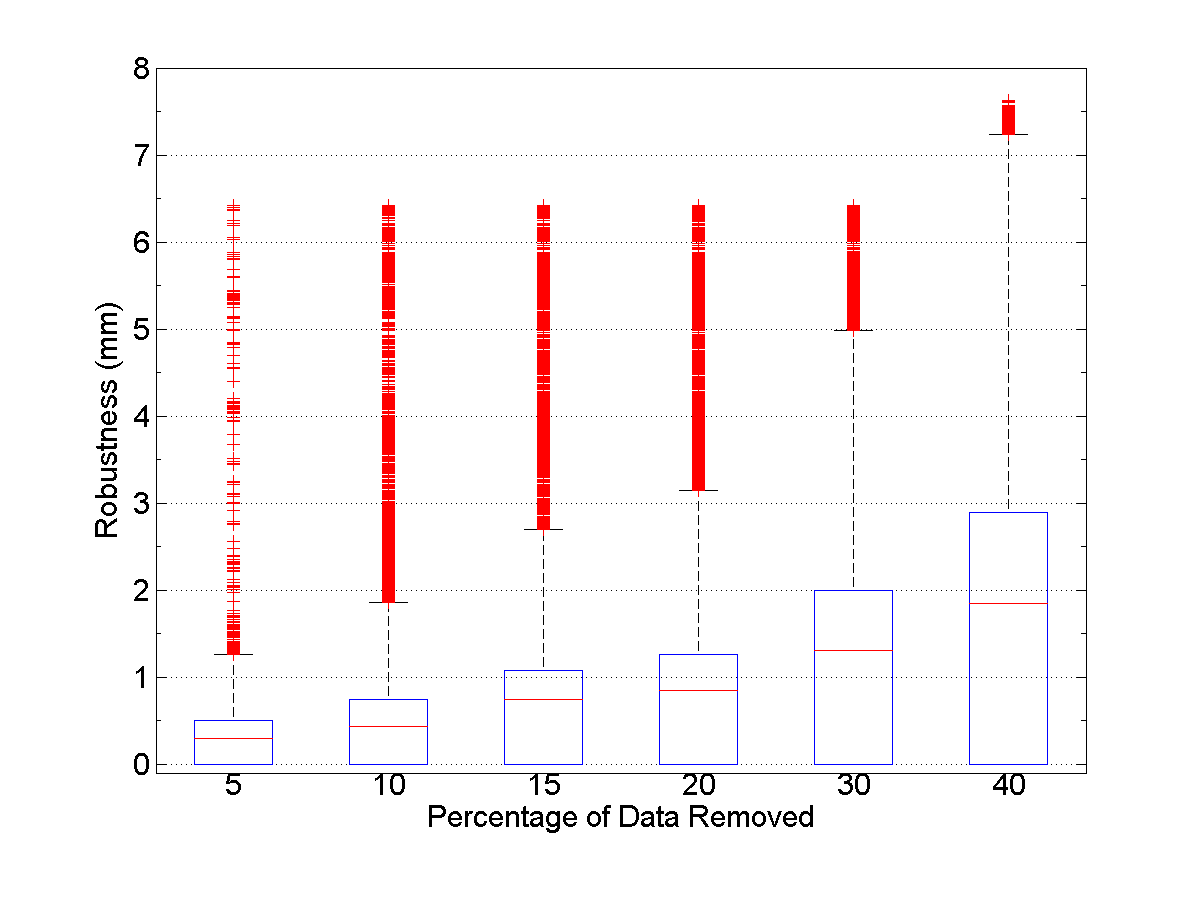
\includegraphics[width=\columnwidth]{images/MissingDataBar}}\\
	\subfloat[][Left to right: Spatial distribution of robustness for SSM-FEM registration when 10\%, 20\% and 40\% of observations are removed.\label{fig:MissingSpatial}]{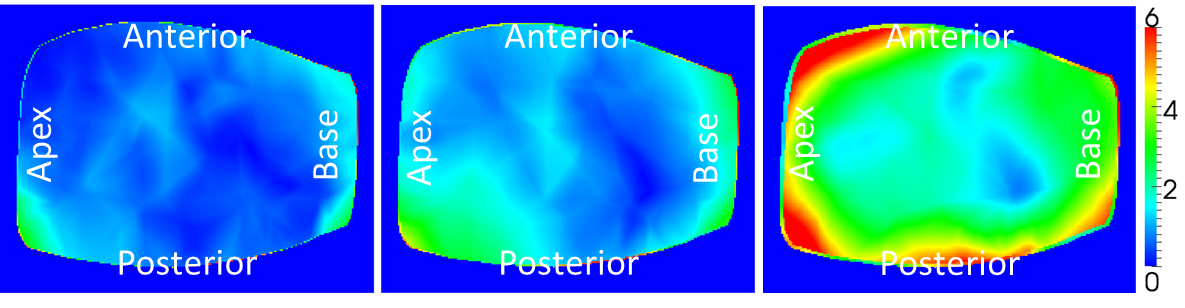
\includegraphics[width=\columnwidth]{images/MissingDataSpatial}}
	\caption{Distribution of robustness as different percentages of observations are removed with $E=5.0$~kPa, $\mu=400$, $\beta=10.0$, and $\nu=0.49$. Sagittal slice of robustness for SSMM-FEM registration when different amounts of observations are removed. For better visualization, distances larger than 6~mm are shown in the same color.}\label{fig:Missing}
\end{figure}
%%%%%%%%%%%%%%%%%%%%%%%%%%%%%%%%%
In the second set of experiments, we investigate the robustness of our method when parts of the observations are missing. This provides a measure of confidence of the TRE in regions where the prostate is not segmented. Robustness is defined as the performance of an algorithm in the presence of disruptive factors~\cite{Jannin02a}. To this end, we systematically removed portions of observation points (i.e. rows of $X_\mathrm{md}$) from both the base and apex (from 2.5\% to 20\% from each). Subsequently, we applied our algorithm to the cropped observations. No points were removed from the SSM surface (i.e rows of $Z$), since we assume that the SSM can be reliably and accurately constructed. In order to quantify the performance, we compared the internal deformation fields computed with missing observations to that without, when deforming from the MR coordinate space to the TRUS space. We explicitly define robustness as the $L_2$ distance of the deformation field computed with missing observations to the deformation field computed when no observations are removed. This implicitly defines robustness as the fidelity of the registration in recovering the same deformation field without missing data, i.e. a smaller value corresponds to a better robustness.

The results of this experiment are shown in Figure~\ref{fig:Missing} for a typical biopsy patient. Excluding outliers in Figure~\ref{fig:MissingBox}, internal deformations stay below $2.0$~mm when $10\%$ of the observations are removed from the SSM-FEM registration. The robustness of SSM-FEM registration progressively declines as more observations in the base and apex regions are removed. As seen in Figure~\ref{fig:MissingSpatial}, the deformation field in the central region of the prostate is more robust to missing data compared to base and apex regions. This is a consequence of the FE model: the central regions are affected by all surrounding tissue, so forces propagated from the boundaries, particularly from the base and apex, are more balanced.  Regions local to the areas of missing data are less constrained, so move more freely due to the implicit surface forces that arise during optimization.

%%%%%%%%%%%%%%%%%%%%%%%%%%%%%%%%%
\subsection{Sensitivity to Regularization Parameters}\label{sec:exp3}
%%%%%%%%%%%%%%%%%%%%%%%%%%%%%%%%%

%%%%%%%%%%%%%%%%%%%%%%%%%%%%%%%%%
\begin{figure*}[t]
	\centering
	\subfloat[][Box-plot distribution of robustness as $\mu$ is perturbed\label{fig:MuBox}]{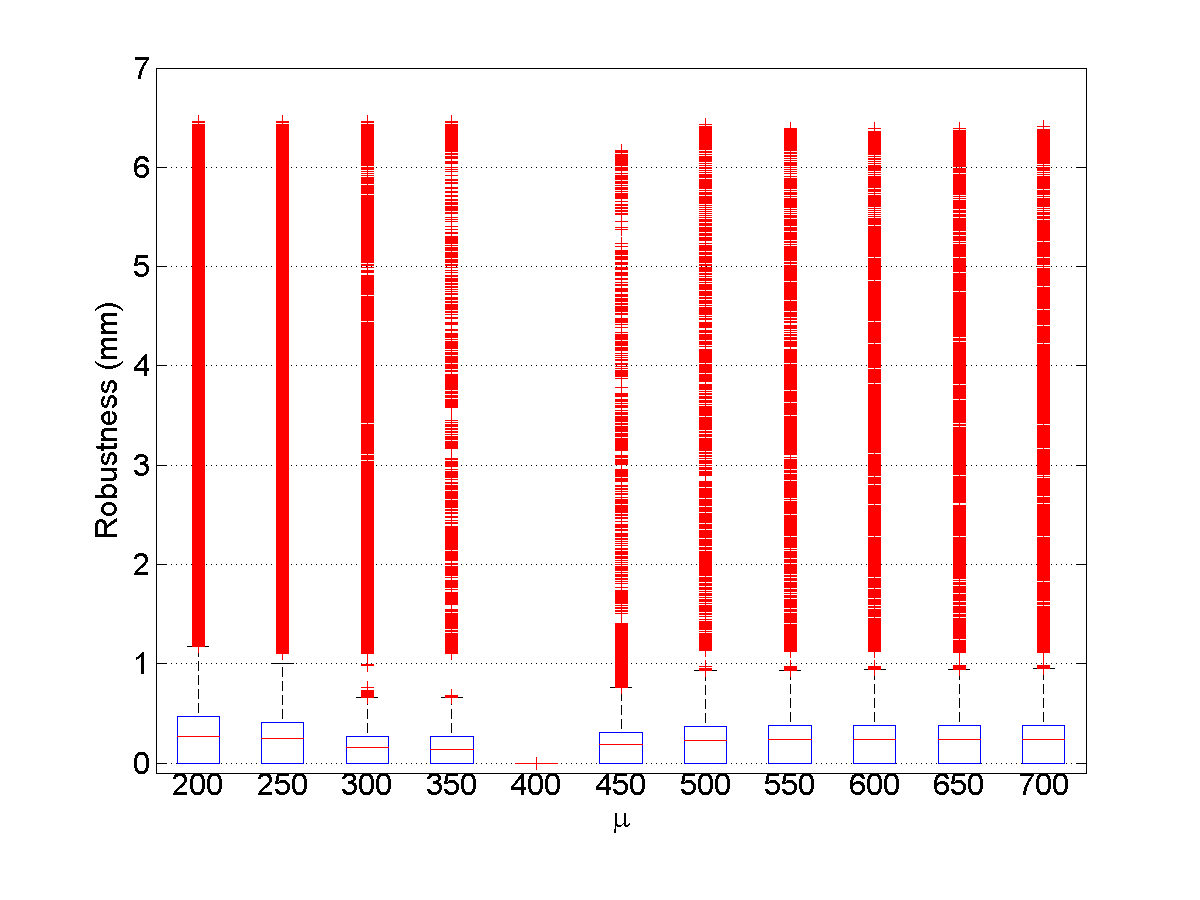
\includegraphics[width=\columnwidth]{images/Boxplot_mu}}
	\hfill
	\subfloat[][Box-plot distribution of robustness as $\beta$ is perturbed\label{fig:BetaBox}]{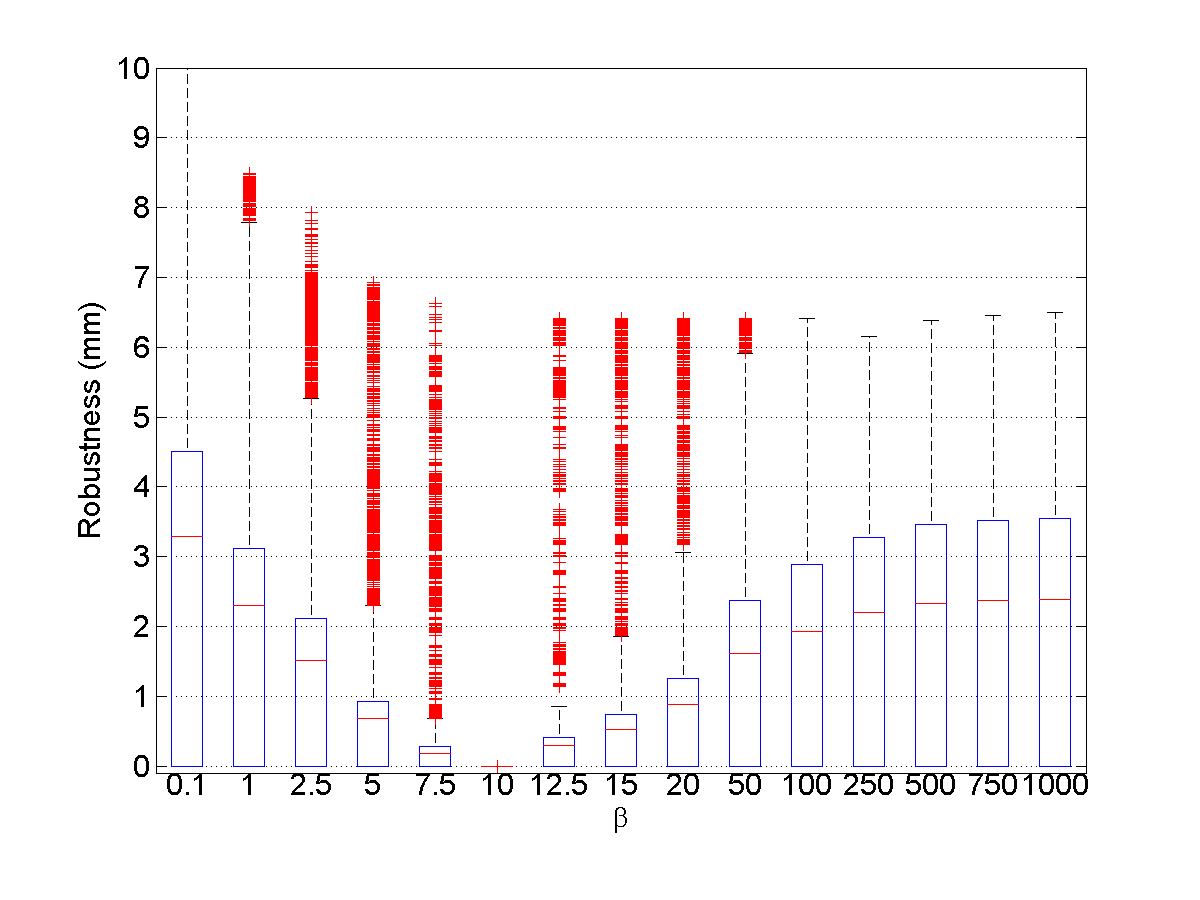
\includegraphics[width=\columnwidth]{images/Boxplot_beta}}
	\\
	\subfloat[][Left to right: Spatial distribution of robustness for SSM-FEM registration when $\mu$ is set to 200, 350 and 550, respectively.\label{fig:MuSpatial}]{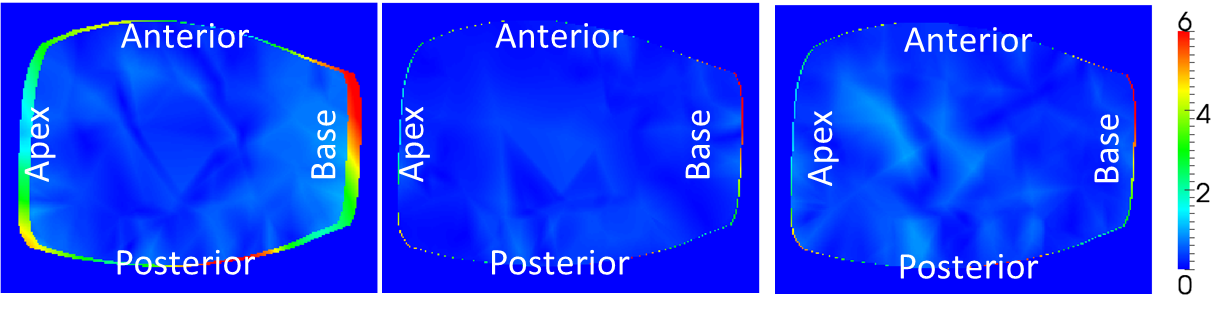
\includegraphics[width=\columnwidth]{images/MuSpatial}}
	\hfill
	\subfloat[][Left to right: Spatial distribution of robustness for SSM-FEM registration when $\beta$ is set to 2.5, 7.5 and 20.0, respectively.\label{fig:BetaSpatial}]{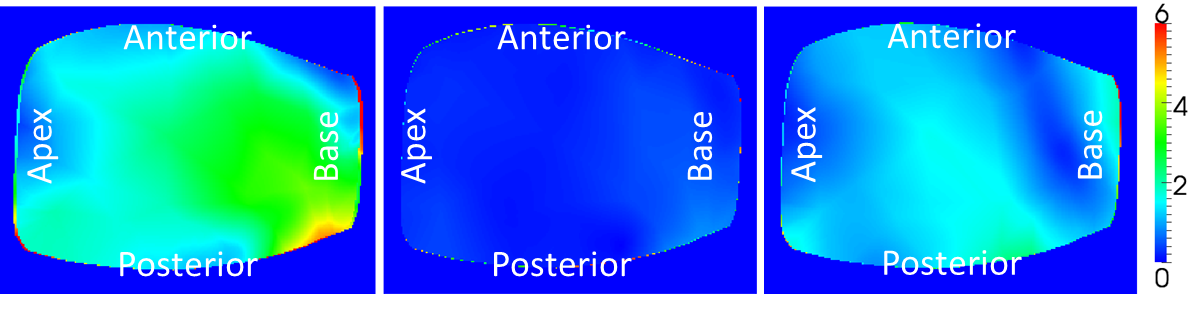
\includegraphics[width=\columnwidth]{images/BetaSpatial}}
	
	\caption{Robustness of SSM-FEM registration for different regularization weights. (a) varying the SSM scale factor, $\mu$. (b) varying the FEM scale factor, $\beta$. Weights are perturbed around parameters which provided the best surface overlap ($E=5.0$~kPa, $\nu=0.49$, $\mu=400$ and $\beta=10.0$). For better visualization contrast, distances larger than 6~mm are shown with the same color.}\label{fig:Perturb}
\end{figure*} 

In the final set of experiments, we investigate robustness of our method to parameters that control the regularizers. Specifically, we investigate the effect of changing the Tikhonov weights (i.e. $\mu$ and $\beta$) on the composition of the MR-TRUS deformation field. We recommend a value of $\nu=0.49$ for Poisson's ratio, since we assume the prostate to maintain a constant volume. We do not investigate the effect of changing the Young's modulus since, under the assumption of homogeneous elasticity, it can be shown that the stiffness matrix is simply scaled by this value.  This allows any further scaling to be captured solely by adjusting $\beta$. As a result, the only two free parameters for the proposed registration algorithm are $\mu$ and $\beta$. In order to examine the sensitivity of our registration method to these parameters, we perturbed the values for these regularization weights: $\mu\in[200,700]$, and $\beta\in[0.1,1000]$.  Results are shown in Figure~\ref{fig:Perturb} for a typical fully segmented prostate.
Figure~\ref{fig:MuBox} shows the sensitivity of the internal deformation field to the Tikhonov weight that controls the SSM shape parameters. The registration seems not to be sensitive to perturbations in this parameter, particularly when compared to the biomechanical regularization weight. For small values, $\mu\leq200.0$, due to the different appearance of the prostate in MR and TRUS surfaces, the registration becomes unstable, and Equation~\eqref{eq:SSM1} produces invalid instances. For large Tikhonov values, $\mu\geq550.0$, the SSM is restricted to instances close to the mean shape. For values between these two extremes, the search space of the registration is restricted to valid instances of the SSM. As seen in Figure~\ref{fig:MuSpatial}, changes in $\mu$ mostly affect the boundary of the prostate; regions interior to the prostate are less sensitive to these perturbations.

As seen in Figure~\ref{fig:BetaBox}, the SSM-FEM registration is much more sensitive to the biomechanical regularization weight. When tuning this parameter, the registration approach exhibited three distinct behaviors. For large values, in this case $\beta\geq50.0$, the FEM is essentially rigid, allowing no further deformation. For very small weights (e.g.~$\beta\leq2.5$) the FEM does not provide any regularization: the surface is allowed to move freely, independently of interior nodes. For values in-between the two extremes, the parameter allows one to trade-off between surface-fitting and resisting internal deformation.

Figure~\ref{fig:BetaSpatial} shows the spatial distribution of robustness for the three different behaviors just described. The deformation field around the mid-gland seems less robust to perturbations in the regularization weight compared to base and apex. 
%\redout{One possible explanation is that the prostate shape is much different due to probe-induced biomechanical forces}.

%%%%%%%%%%%%%%%%%%%%%%%%%%%%%%%%%
\section{Discussion and Conclusions}
%%%%%%%%%%%%%%%%%%%%%%%%%%%%%%%%%
In this paper, we presented a novel non-rigid surface-based registration approach that is robust to missing data.  The method uses a statistical shape model as an intermediary in order to register two partial surfaces.  The SSM introduces geometric prior knowledge, allowing for varying shapes across a population.  To account for physical deformations, we introduce a finite-element based regularizer.  This lets the SSM deform, accounting for differences in biomechanical strain states between the observed partial surfaces.

The proposed registration algorithm converges within thirty seconds on a regular desktop PC. We showed the internal deformation found through our proposed method to be robust up to $2.0$~mm when 10\% of observations are removed. A great advantage of the algorithm is that it estimates point-correspondences, nodal displacements, shape and pose parameters in a single minimization framework.  This is one of the contributing factors to the efficiency of the algorithm.  We also obtain a full volumetric deformation field for the object of interest as a by-product of the regularization.  This is in contrast to many existing surface-based approaches, where a volumetric deformation needs to be estimated from surface deformations in an additional post-processing step.

The most time-consuming portion of the registration method is the FE meshing component, which is called every time a new SSM shape instance is generated. If further speed-up is necessary, it is possible to perform meshing only when the generated instance differs significantly from the previous iteration. Another shortcoming of our algorithm is that it requires the MR and TRUS to be segmented prior to the registration. While the MR can typically be segmented ahead of time, the 3D-TRUS needs to be segmented within minutes due to clinical requirements if the method is to be used in an image-guided intervention. One possible solution is to use an existing fast, semi-automatic segmentation method~\cite{Qiu12a}. Since our algorithm is designed to handle partial surfaces, and is robust to missing data, we suggest to only segment regions in which the boundary of the anatomy can be clearly distinguished, such as in the mid-gland. This can also help speed up the segmentation process.

In Section~\ref{sec:exp1} we investigated the performance of our registration method using fiducial pairs found in the interior of the prostate. The SSM-FEM algorithm yields a statistically significant improvement following registration ($1.8$~mm compared to rigid registration alone). While the improvement is small, it should be compared to the acceptable error bounds of a targeted biopsy system. With a TRE of $2.5$~mm, one can obtain a confidence interval corresponding to two standard deviations from the mean (i.e.~the estimated true center of the tumor). If this requirement is met, then 95\% of registered targets come within the clinically significant $5$~mm radius~\cite{Karnik10a}. Our improvement on TRE brings us closer to the acceptable error bounds of a targeted biopsy system.

In this manuscript, we used an isotropic Gaussian mixture model to represent surface nodes on the SSM, and applied an expectation-maximization framework to estimate the correspondences between SSM and TRUS/MR surfaces. While isotropic GMMs have been shown to be effective in rejecting noise/outliers~\cite{Myronenko10a}, this assumption breaks in the presence of anisotropic noise. To tackle this issue, similar to Zheng~\cite{Zheng13a}, the proposed method can be easily extended to include anisotropic GMMs in an expectation conditional maximization (ECM) framework~\cite{Horaud11a}.

While the set of observations in this manuscript was limited to registering images from two modalities, the proposed method is trivially extended to concurrently register more than two surfaces. Such a situation may arise when the patient is scheduled for a re-biopsy, and it is desirable to simultaneously register MR, the previous TRUS, and the current TRUS surfaces. This would enable the radiologist to avoid areas that in the previous biopsy were found to be cancer-free and enable re-sampling areas that are prone to develop cancer, such as BPH and suspicious MR regions.  The extension is accomplished by modifying the objective function in Equation \eqref{eq:objTotal2} to sum over further observations.

The implicit assumption when using the SSM as a ``starting shape'' for computing biomechanical deformations is that it represents the prostate ``at rest''.  This assumption is not true in general, since there will always be some biomechanical forces present in the training population (e.g.~pressure from the bladder, gravity, probes/endorecal coils).  Ideally, the training images would be acquired under conditions where these forces are minimized.  The training population in our study is a compromise in size, segmentation accuracy, and initial biomechanical forces.  To account for errors caused by existing deformations in the training data, an initial strain field can be estimated.  This can be accomplished by measuring or estimating any external forces (e.g.~from a force sensor on a transrectal probe), and back-solving for the initial strain \cite{pelteret2012a}.
%If needed, the error caused by any existing strains
%\comment{talk about the SSM, rest shape argument, brachiotherapy has some initial deformation due to probe... we are assuming this is a ``rest'' (undeformed) shape... image undeformed... estimating initial strain field (strain imaging... either compensate, or estimate undeformed) , image when minimally deformed }

In this paper, we used a linear material in the construction of the prostate finite element model. However for most soft tissue, some degree viscoleastic, poroelastic, anisotropic and nonlinear response is expected when a mechanical force is applied. If the nonlinear response is significant, non-linear models, such as the Mooney-Rivlin material \cite{Rivlin48}, can easily be included.  This requires linearizing the strain energy about the current deformation state and updating the stiffness matrix at each iteration. This will also introduce an additional synthetic force to be added to the objective function that encodes the current state.  We also currently assume homogenous tissue parameters.  Any inhomogeneities in tissue parameters (e.g. Young's Modulus) can easily be incorporated in the computation of the FE stiffness matrix.  If additional elastic information about the elastic properties of the tissue is available (e.g. through elastography), this would need to be mapped to the space of the SSM instance.  Such a mapping can be easily incorporated into our framework by segmenting the boundary of the prostate in the elastography image, and using this as an additional observation to be registered.  We would then initialize the material parameter to a constant value, then update local stiffness as the registration proceeds.

Our probabilistic algorithm is based on very simple concepts: soft-correspondences via Gaussian mixture models, geometric prior knowledge provided by a statistical shape model, and biomechanical regularization based on a linearized finite element model.  The soft correspondences make it robust to noise and missing data points; the SSM provides potentially missing geometric information when boundaries of anatomical regions are not clear in images; and the FEM provides flexibility, allowing the shape to deform to account for soft-tissue motion between acquisitions.  While the application in this paper is MR-TRUS registration for prostate biopsies, the method is very general and can be used to concurrently register any set of surfaces or partial surfaces, regardless of modality.

%%%%%%%%%%%%%%%%%%%%%%%%%%%%%%%%%
\section*{Acknowledgements}
%%%%%%%%%%%%%%%%%%%%%%%%%%%%%%%%%
This work was supported by the Natural Sciences and Engineering Research Council of Canada (NSERC), the Canadian Institutes of Health Research (CIHR), and the University of British Columbia.
%%%%%%%%%%%%%%%%%%%%%%%%%%%%%%%%%
\appendices
%%%%%%%%%%%%%%%%%%%%%%%%%%%%%%%%%

\section{Derivation of Shape Parameters}\label{sec:app:ssm}
%%%%%%%%%%%%%%%%%%%%%%%%%%%%%%%%%
To minimize Equation~\eqref{eq:objTotal2} \wrt\ shape parameters, conditioned by observations in both modalities, we first ignore terms independent of $b$:
%%%%%%%%%%%%%%%%%%%%%%%%%%%%%%%%%
\begin{align}\label{eq:SSMD1}
  \mathcal{E}(b) = & \sum_\mathrm{md}\dfrac{1}{2\sigma^2_\mathrm{md}}\!\sum_{m,n=1}^{M,N_\mathrm{md}}\!P_\mathrm{md}\left\|x^\mathrm{md}_n-sR\left(z^\mathrm{md}_m+\Psi_mb\right)-t\right\|^2\notag\\
  & \quad + \frac{\mu}{2}\trans{b}\Lambda{b},
\end{align}
%%%%%%%%%%%%%%%%%%%%%%%%%%%%%%%%%
where $\mathrm{md}\in\{\mathrm{MR},\mathrm{US}\}$, $P_\mathrm{md}=P(z_m|x^\mathrm{md}_n)$ and $z^\mathrm{md}_m=z_m+v^\mathrm{md}_m$. We can expand Equation~\eqref{eq:SSMD1} and re-write it in a rasterized form:
%%%%%%%%%%%%%%%%%%%%%%%%%%%%%%%%%
\begin{align}\label{eq:SSMD2}
  \mathcal{E}(b) = & \sum_\mathrm{md}\dfrac{1}{2\sigma^2_\mathrm{md}}\left[N^\mathrm{md}_p\trans{t}_\mathrm{md}t_\mathrm{md}+\trans{\vec{x}_\mathrm{md}}\diag(\trans{\tilde{P}_\mathrm{md}}1)\vec{x}_\mathrm{md}\right.\notag\\
  & \quad -2\trans{t}_\mathrm{md}\trans{\hat{I}}\diag(\trans{\tilde{P}_\mathrm{md}}1)\vec{x}_\mathrm{md}\notag\\
  & \quad +s^2_\mathrm{md}\;\trans{(\vec{z}_\mathrm{md}+{\Psi}b)}\diag(\tilde{P}_\mathrm{md}1)(\vec{z}_\mathrm{md}+{\Psi}b)\notag\\
  & \quad +2s_\mathrm{md}\;\trans{t}_\mathrm{md}R_\mathrm{md}\trans{\tilde{I}}\diag(\tilde{P}_\mathrm{md}1)(\vec{z}_\mathrm{md}+{\Psi}b)\notag\\
  & \quad \left.-2s_\mathrm{md}\;\trans{\vec{x}_\mathrm{md}}\trans{\tilde{P}_\mathrm{md}}\tilde{R}_\mathrm{md}(\vec{z}_\mathrm{md}+{\Psi}b)\right]\notag\\
  & \quad + \frac{\mu}{2}\trans{b}\Lambda{b},
\end{align}
%%%%%%%%%%%%%%%%%%%%%%%%%%%%%%%%%
where $\trans{\hat{I}} = \begin{bmatrix} I_{D\times D} & \cdots & I_{D\times D} \end{bmatrix}_{D\times ND}$. The matrix $\tilde{P}_\mathrm{md}=\kron{(P_\mathrm{md},I_{D\times{D}})}$ is the Kronecker-delta product of the correspondence probability matrix with an identity matrix, so it can be applied to a concatenation of all $(x,y,z)$ coordinates of input points.  Differentiation \wrt\ $b$ results in:
%%%%%%%%%%%%%%%%%%%%%%%%%%%%%%%%%
\begin{align}\label{eq:SSMD3}
    \di{\mathcal{E}(b)}{b} = & \mu\Lambda{b}+\sum_\mathrm{md}\dfrac{1}{2\sigma^2_\mathrm{md}}\left[2s^2_\mathrm{md}\trans{\Psi}\diag(\tilde{P}_\mathrm{md}1){\Psi}b\right.\notag\\
  & \quad +2s^2_\mathrm{md}\;\trans{\Psi}\diag(\tilde{P}_\mathrm{md}1)\vec{z}_\mathrm{md}\notag\\
  & \quad +2s_\mathrm{md}\;\trans{\Psi}\diag(\tilde{P}_\mathrm{md}1)\tilde{I}\trans{R}_\mathrm{md}t_\mathrm{md}\notag\\
  & \quad \left.-2s_\mathrm{md}\;\trans{\Psi}\tilde{R}_\mathrm{md}\tilde{P}_\mathrm{md}\vec{x}_\mathrm{md}\right].
\end{align}
%%%%%%%%%%%%%%%%%%%%%%%%%%%%%%%%%
Setting Equation~\eqref{eq:SSMD3} to zero yields the final set of linear equations:
\begin{equation*}
\Gamma_{\mathrm{SSM}}b = \Upsilon_\mathrm{SSM},
\end{equation*}
%%%%%%%%%%%%%%%%%%%%%%%%%%%%%%%%%%%%%%
with
%%%%%%%%%%%%%%%%%%%%%%%%%%%%%%%%%%%%%%
\begin{align*}
\Gamma_{\mathrm{SSM}} = & \mu\Lambda + \sum_\mathrm{md}\frac{s^2_\mathrm{md}}{\sigma^2_\mathrm{md}}\trans{\Psi}\diag(\tilde{P}_\mathrm{md}1)\Psi,\\
 \Upsilon_{\mathrm{SSM}} = & \sum_{\mathrm{md}}\frac{s_\mathrm{md}}{\sigma^2_\mathrm{md}}\left(\trans{\Psi}\trans{\tilde{R}}_\mathrm{md}\tilde{P}_\mathrm{md}\vec{x}_\mathrm{md}\right.\nonumber\\
 & \;\; \left.-\trans{\Psi}\diag(\tilde{P}_\mathrm{md}1)\!\!\left(s_\mathrm{md}(\vec{z}+\vec{v}_\mathrm{md})+\tilde{I}\trans{R}_\mathrm{md}t_\mathrm{md}\right)\right)\nonumber.
\end{align*}
%%%%%%%%%%%%%%%%%%%%%%%%%%%%%%%%%

\section{Derivation of FE Nodal Displacements}\label{sec:app:fem}
%%%%%%%%%%%%%%%%%%%%%%%%%%%%%%%%%
Minimization of Equation~\eqref{eq:objTotal2} \wrt\ nodal displacements in each modality is equivalent to registering the SSM instance to each observation independently. To avoid clutter, we drop the modality subscript, $\mathrm{md}$, throughout this section.

Limiting to a single modality and ignoring terms independent of $U$, Equation~\eqref{eq:objTotal2} can be written as:
%%%%%%%%%%%%%%%%%%%%%%%%%%%%%%%%%
\begin{align}\label{eq:FE1}
  \mathcal{E}(U) = & \dfrac{1}{2\sigma^2}\sum_{m,n=1}^{M,N}P(z_m|x_n)\left\|x_n-sR\left(y_m+\Phi_mU\right)-t\right\|^2\notag\\
  & \quad + \dfrac{\beta}{2}\trans{\vec{u}}K\vec{u},
\end{align}
%%%%%%%%%%%%%%%%%%%%%%%%%%%%%%%%%
where $\vec{u}=\trans{(u_{11},\ldots,u_{1D},\ldots,u_{JD})}$ is the rasterized representation of $U$. Written in matrix form, this is equivalent to
%%%%%%%%%%%%%%%%%%%%%%%%%%%%%%%%%
\begin{align}\label{eq:FE2}
    \mathcal{E}(U) & = \dfrac{1}{2\sigma^2}\left[N_P\trans{t}t + \trace\left(\trans{X}\diag(\trans{P}1)X\right)-2\trans{t}\trans{X}\trans{P}1\right.\notag\\
    & \qquad +s^2\;\trace\left(\trans{(Y+\Phi U)}\diag(P1)(Y+\Phi U)\right) \notag\\
    & \qquad + 2s\;\trans{t}R\trans{(Y+ \Phi U)}P1\notag\\
    & \qquad \left.-2s\;\trace\left(\trans{X}\trans{P}(Y+\Phi U)\trans{R}\right)\right]\notag\\
    & \qquad + \dfrac{\beta}{2}\trans{\vec{u}}K\vec{u},
\end{align}
%%%%%%%%%%%%%%%%%%%%%%%%%%%%%%%%%
where $\trace(\cdot)$ denotes the trace of a square matrix. To simplify the derivation, we can rewrite Equation~\eqref{eq:FE2} in a rasterized form:
%%%%%%%%%%%%%%%%%%%%%%%%%%%%%%%%%
\begin{align}\label{eq:FE3}
    \mathcal{E}(\vec{u}) & = \dfrac{1}{2\sigma^2}\left[N_P\trans{t}t + \trans{\vec{x}}\diag(\trans{\tilde{P}}1)\vec{x}-2\trans{t}\trans{\hat{I}}\diag(\trans{\tilde{P}}1)\vec{x}\right.\notag\\
    & \qquad\qquad + s^2\;\trans{(\vec{y}+\tilde{\Phi}\vec{u})}\diag(\tilde{P}1)(\vec{y}+\tilde{\Phi}\vec{u})\notag\\
    & \qquad\qquad +2s\;\trans{t}R\trans{\tilde{I}}\diag(\tilde{P}1)(\vec{y}+\tilde{\Phi}\vec{u})\notag\\
    & \qquad\qquad \left.-2s\;\trans{\vec{x}}\trans{\tilde{P}}\tilde{R}(\vec{y}+\tilde{\Phi}\vec{u})\right] + \dfrac{\beta}{2}\trans{\vec{u}}K\vec{u},
\end{align}
%%%%%%%%%%%%%%%%%%%%%%%%%%%%%%%%%
where $\trans{\hat{I}} = \begin{bmatrix} I_{D\times D} & \cdots & I_{D\times D} \end{bmatrix}_{D\times ND}$. Excluding terms independent of $\vec{u}$, this reduces to
%%%%%%%%%%%%%%%%%%%%%%%%%%%%%%%%%
\begin{align}\label{eq:FE4}
    \mathcal{E}(\vec{u}) & = \dfrac{s^2}{2\sigma^2}\trans{\vec{u}}\trans{\tilde{\Phi}}\diag(\tilde{P}1)\tilde{\Phi}\vec{u} + \dfrac{\beta}{2}\trans{\vec{u}}K\vec{u}\\
    & \quad + \dfrac{1}{\sigma^2}\left[\left(s^2\trans{\vec{y}}+s\;\trans{t}R\trans{\tilde{I}}\right)
        \diag(\tilde{P}1)-s\;\trans{\vec{x}}\trans{\tilde{P}}\tilde{R}\right]\tilde{\Phi}\vec{u}\notag
\end{align}
%%%%%%%%%%%%%%%%%%%%%%%%%%%%%%%%%
Differentiating with respect to $\vec{u}$ results in:
%%%%%%%%%%%%%%%%%%%%%%%%%%%%%%%%%
\begin{align}\label{eq:FE5}
    \di{\mathcal{E}(\vec{u})}{\vec{u}} & = \left[\dfrac{s^2}{\sigma^2}\trans{\tilde{\Phi}}\diag(\tilde{P}1)\tilde{\Phi} + \beta K\right]\vec{u}\\
        & \quad + \dfrac{1}{\sigma^2}\left[\trans{\tilde{\Phi}}\diag(\tilde{P}1)\!\left(s^2\vec{y}+s\tilde{I}\trans{R}t\right)
        -s\trans{\tilde{\Phi}}\trans{\tilde{R}}\tilde{P}\vec{x}\right].\notag
\end{align}
%%%%%%%%%%%%%%%%%%%%%%%%%%%%%%%%%
Setting $\partial\mathcal{E}(\vec{u})/\partial\vec{u}\!=\!0$ results in the desired system of linear equations:
%%%%%%%%%%%%%%%%%%%%%%%%%%%%%%%%%
\begin{align*}
    \Gamma_\mathrm{FEM}\vec{u} &= \Upsilon_\mathrm{FEM},
\end{align*}
%%%%%%%%%%%%%%%%%%%%%%%%%%%%%%%%%
where
%%%%%%%%%%%%%%%%%%%%%%%%%%%%%%%%%
\begin{align*}
\Gamma_\mathrm{FEM} &= \beta \sigma^2K + s^2\trans{\tilde{\Phi}}\diag(\tilde{P}1)\tilde{\Phi}\\
    \Upsilon_\mathrm{FEM} &= s\trans{\tilde{\Phi}}\trans{\tilde{R}}\tilde{P}\vec{x} - \trans{\tilde{\Phi}}\diag(\tilde{P}1)\left(s^2\vec{y}+s\tilde{I}\trans{R}t\right).\notag
\end{align*}
%%%%%%%%%%%%%%%%%%%%%%%%%%%%%%%%%

\ifCLASSOPTIONcaptionsoff
  \newpage
\fi

\bibliography{tmi2}
\bibliographystyle{IEEEtranN}

\end{document}

%%%%%%%%%%%%%%%%%%%%%%%%%%%%%%%%%
% SSM compactness figure
%\begin{figure}[t]
%	\centering
%	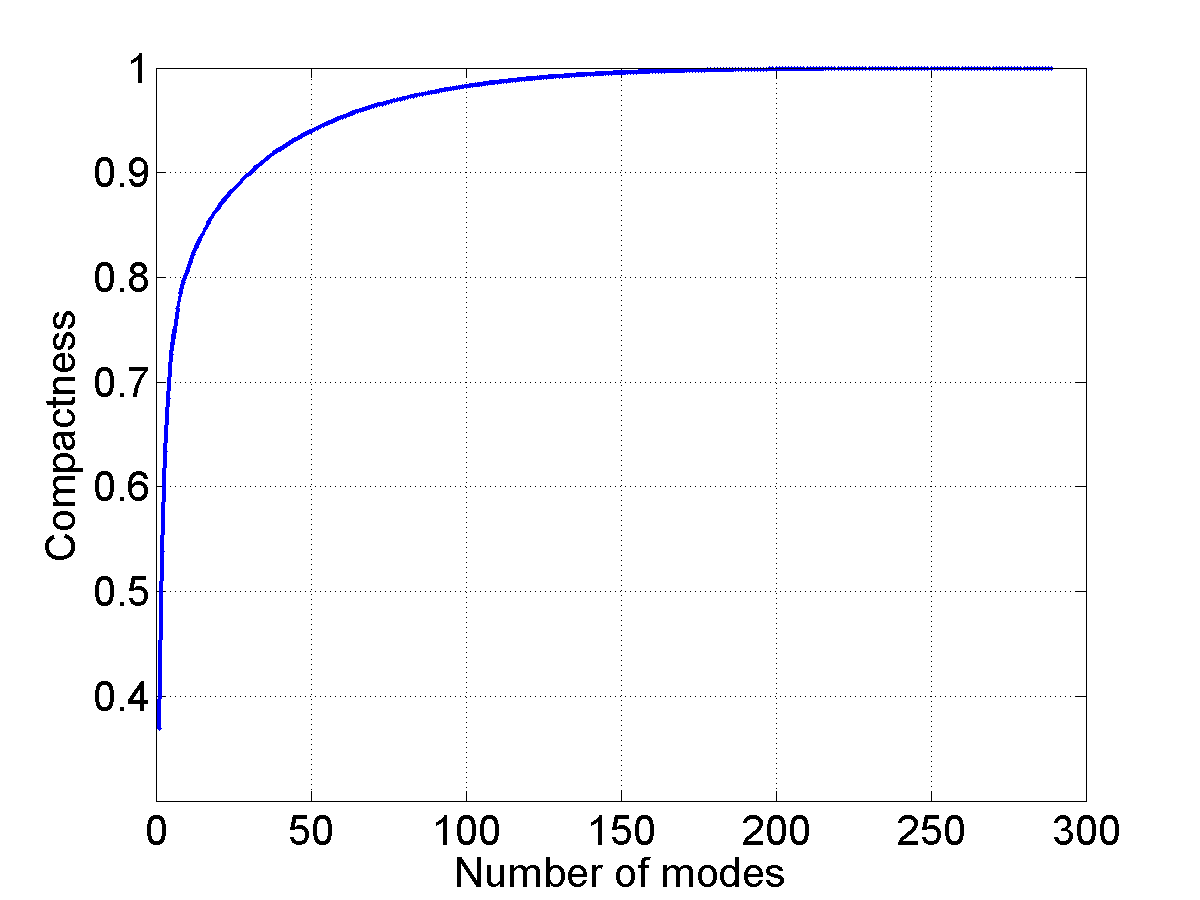
\includegraphics[width=\columnwidth]{images/compactness}
% \caption{Compactness of the constructed SSM given the first $L$ principal modes of variation.}\label{fig:SSM_compactness}
%\end{figure}
%%%%%%%%%%%%%%%%%%%%%%%%%%%%%%%%%